\documentclass[11pt]{article}

\usepackage[french]{babel}
\usepackage[utf8]{inputenc}

\usepackage[T1]{fontenc}


\usepackage{booktabs}
%% Camille, change the color as you wish
\usepackage[pdftex,dvipsnames,usenames]{xcolor}
\usepackage[pdftex,colorlinks=true,urlcolor=ForestGreen,citecolor=Blue,linkcolor=BrickRed]{hyperref} % Must be loaded before cleveref
\usepackage{paralist}


\usepackage{graphicx}
\graphicspath{{./fig/}}

\usepackage{amsmath,amsthm,amssymb}
\usepackage[normalem]{ulem}

\textwidth 16cm
%\textheight 22cm
\evensidemargin 0cm
\oddsidemargin 0cm

\usepackage{colors}
\usepackage{encarts}
\usepackage{tikzstyles}
\usepackage{theoremes}
\usepackage{macros}

\title{Activité : Partition}
\date{}

\begin{document}

\maketitle
\tableofcontents

\section{Description du problème}

  \begin{definition}{Partition d'un ensemble}
    Un \emph{multiensemble} (parfois appelé sac) est un ensemble dans lequel chaque élément peut apparaître plusieurs fois.

    Soit un multiensemble $S$ de $n$ entiers naturels.

    $$S = \{s_i\ |\ s_i > 0\}_{1\leq i \leq n}.$$

    Une \emph{(bi)partition} de $S$ est constituée de deux sous-multiensembles $S_1$ et $S_2$ tels que :
    \begin{itemize}
      \item $S_1$ et $S_2$ sont non vides:  $S_1 \neq \emptyset$ et $S_2 \neq \emptyset$ ;
      \item $S_1$ et $S_2$ sont disjoints:  $S_1 \cap S_2 = \emptyset$ ;
      \item $S_1$ et $S_2$ recouvrent $S$:  $S_1 \cup S_2 = S$ ;
    \end{itemize}
  \end{definition}

  \begin{exemple}{Partition d'un ensemble}
    Soit un multiensemble $S = \{1,2,3,4,5\}$.
    \begin{itemize}
      \item Les multiensembles $S_1$ et $S_2$ forment une partition de $S$.
        \begin{itemize}
          \item $S_1 = \{1\}$ et $S_2 = \{2,3,4,5\}$
          \item $S_1 = \{2, 4\}$ et $S_2 = \{1,3,5\}$
        \end{itemize}
      \item Les multiensembles $S_1$ et $S_2$ ne forment pas une partition de $S$.
        \begin{itemize}
          \item $S_1 = \{1,2,3,4,5\}$ et $S_2 = \emptyset$, car $S_2$ est vide.
          \item $S_1 = \{1,2,3\}$ et $S_2 = \{3,4,5\}$, car leur intersection est non vide.
          \item $S_2 = \{1,2\}$ et $S_2 = \{4, 5\}$, car 3 est dans 4, mais n'appartient ni à $S_1$ ni à $S_2$.
        \end{itemize}
    \end{itemize}
  \end{exemple}

  \begin{definition}{Partition parfaite d'un multiensemble pair}
    Un multiensemble d'entiers $S$ est dit \emph{pair} si la somme des entiers de $S$ est pair.

    Une \emph{partition parfaite} d'un multiensemble pair est une partition telle que la valeur absolue de la différence entre la somme des entiers de $S_1$ et la somme des entiers de $S_2$ est 0.
  \end{definition}

  \begin{exemple}{Partition parfaite d'un multiensemble pair}
    $S = \{1,2,3,4\}$ est un multiensemble pair.
    \begin{itemize}
      \item $S_1 = \{1,3\}$ et $S_2 = \{2,4\}$ ne forment pas une partition parfaite.
      \item $S_1 = \{1,4\}$ et $S_2 = \{2,3\}$ forment une partition parfaite.
    \end{itemize}
  \end{exemple}

  \begin{definition}{Partition parfaite d'un multiensemble impair}
    Un multiensemble d'entiers $S$ est dit \emph{impair} si la somme des entiers de $S$ est impair.

    Une \emph{partition parfaite} d'un multiensemble impair est une partition telle que la valeur absolue de la différence entre la somme des entiers de $S_1$ et la somme des entiers de $S_2$ est 1.
  \end{definition}

  \begin{exemple}{Partition parfaite d'un multiensemble impair}
    $S = \{1,2,3,4, 5\}$ est un multiensemble impair.

    \begin{itemize}
      \item $S_1 = \{2, 4\}$ et $S_2 = \{1,3,5\}$ ne forment pas une partition parfaite.
      \item $S_1 = \{1, 2, 5\}$ et $S_2 = \{3,4\}$ forment une partition parfaite.
    \end{itemize}
  \end{exemple}

  \begin{definition}{Problème de partitionnement}
  En informatique, le problème de partitionnement consiste à déterminer si une partition parfaite d'un ensembles d'entiers existe. C'est un problème \emph{NP-complet}. Cependant, il existe plusieurs algorithmes qui résolvent efficacement le problème que ce soit de manière approchée ou optimale. Pour ces raisons, il est réputé ``le plus facile des problèmes difficiles" \cite{Mertens2003}.
\end{definition}
  % Le problème de partitionnement se décline aussi en problème d'optimisation dans lequel on recherche une partition minimisant la valeur absolue de la différence entre la somme des entiers des deux sous-ensembles de la partition.
  % Ce problème d'optimisation est \emph{NP-difficile}.


\section{Partition parfaite des entiers de 1 à $n$}

  \begin{exercice}{}
    Trouver une partition parfaite des entiers de 1 à $n$ pour $n =4, 5, 6, 7, 8$.
  \end{exercice}


  \begin{figure}[htbp]
    \centering
    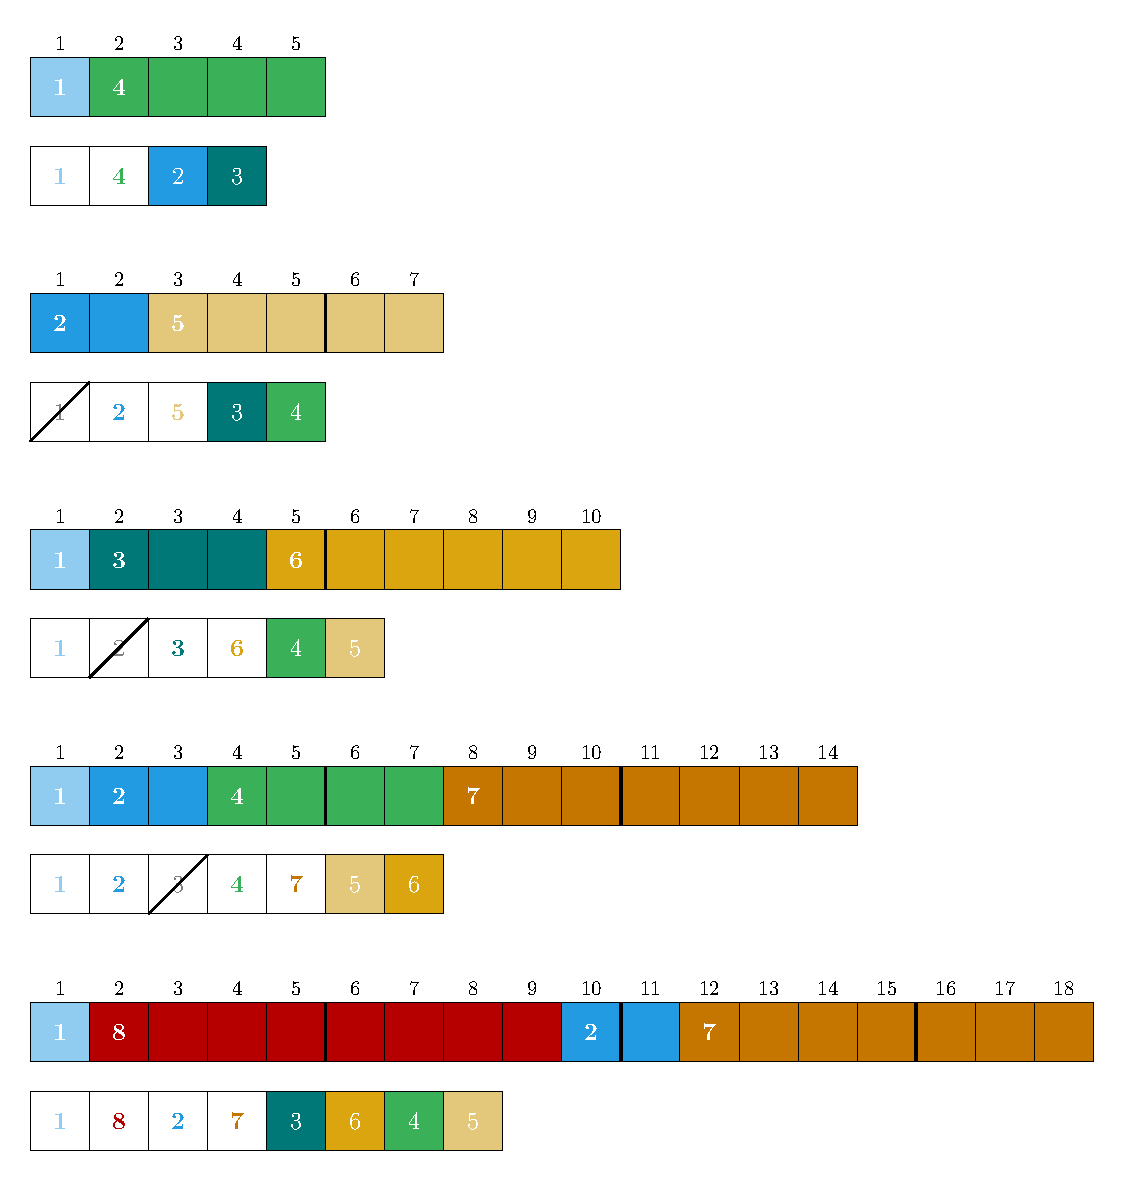
\includegraphics[width=0.6\linewidth]{partition-8.pdf}
    \caption{Partition parfaite des entiers de 1 à $n$.}
  \end{figure}


  \begin{definition}{Algorithme}
    Un \emph{algorithme} répond à un problème. Il est composé d’un ensemble d’étapes simples nécessaires à la résolution, dont le nombre varie en fonction de la taille des données.
  \end{definition}

  \begin{remarque}{}
    Plusieurs algorithmes peuvent répondre à un même problème.
  \end{remarque}

  \begin{remarque}{}
    Un algorithme peut répondre à plusieurs problèmes.
  \end{remarque}

  \begin{exercice}{}
    Donner un algorithme pour trouver une partition parfaite des entiers de 1 à $n$.
  \end{exercice}

  \begin{indice}
    Distinguer les cas en fonction du reste $r$ de la division euclidienne de $n$ par 4. C'est-à-dire qu'il existe $k \geq 0$ et $0 \leq r \leq 3$ tels quel $n = 4 \times k + r$.
    % \begin{tabular}{|*{5}{c |}}
    %   \hline
    %   1 & 2 & $\cdots$ & $p-1$ & $p$\\
    %   $2p$ & $2p-1$ & $\cdots$ & $p+2$ & $p+1$\\\hline
    % \end{tabular}
    % Que remarquez-vous pour chacune des colonnes de ce tableau ?
  \end{indice}


  \begin{algorithme}{Partition parfaite des entiers de 1 à $n$.}
    \begin{itemize}
    \item Soit $n = 4 \times k + r$ le quotient $k$ et le reste $r$ ($0 \leq r \leq 3$) de la division euclidienne de $n$ par 4.
      \begin{itemize}
      \item Si $r=1$, alors éliminer l'objet 1.
      \item Si $r=2$, alors ranger l'objet 1 et éliminer l'objet 2.
      \item Si $r=3$, alors ranger les objets 1 et 2 et éliminer l'objet 3.
      \end{itemize}
  \item Répéter $2 \times k$ fois l'action suivante \\ (ou de manière équivalente, répéter tant que le sac n'est pas rempli) :
    \begin{itemize}
    \item ranger le plus petit et le plus grand objet.
    \end{itemize}
  \end{itemize}
  \end{algorithme}

\begin{remarque}{}
    Ce problème admet une symétrie évidente puisque l'on peut inverser la partition, c'est-à-dire échanger les ensembles $S_1$ et $S_2$.
    De manière générale, on peut toujours échanger des objets entre $S_1$ et $S_2$ si cela ne change pas leurs sommes.
  \end{remarque}


\begin{exercice}{}
  \begin{itemize}
  \item Trouver une partition parfaite des entiers de 1 à 16.
  \item Remarquez que toutes les paires d'objets formées par l'algorithme ont la même somme.
    Trouvez d'autres partitions parfaites par échanges successifs.
  \end{itemize}

\end{exercice}

  % \begin{solution}
  %   Dans l'indice on remarque que la somme des nombres de chaque colonne est la même $2p + 1$.

  %   Quand $p$ est pair on met les nombres des $\frac{p}{2}$ premières colonnes dans un ensemble et ceux des $\frac{p}{2}$ colonnes suivantes dans l'autre ensemble. Les deux ensembles ont donc la même somme. Soit

  %   $$\begin{align*}
  %     S_1 = & \left\{1, 2, \dots, \frac{p}{2}, 2p - \frac{p}{2}+1, 2p - \frac{p}{2}+2, \dots, 2p\right\}\\
  %     S_2 = & \left\{\frac{p}{2} + 1, \frac{p}{2} + 2, \dots, 2p - \frac{p}{2}\right\}.
  %   \end{align*}$$

  %   Quand $p$ est impair on met les nombres des $\frac{p - 1}{2}$ premières colonnes dans un ensemble et ceux des $\frac{p - 1}{2}$ colonnes suivantes dans l'autre ensemble. Il reste la dernière colonne contenant $p$ et $p+1$, on met donc $p$ dans $S_1$ et $p+1$ dans $S_2$. Soit

  %   $$\begin{align*}
  %     S_1 = & \left\{1, 2, \dots, \frac{p-1}{2}, p, 2p - \frac{p-1}{2}+1, 2p - \frac{p-1}{2}+2, \dots, 2p\right\}\\
  %     S_2 = & \left\{\frac{p-1}{2} + 1, \frac{p-1}{2} + 2, \dots, p-1, p+1, p+2, \dots, 2p - \frac{p-1}{2}\right\}.
  %   \end{align*}$$
  % \end{solution}

  % \begin{exercice}{}
  %   Généraliser pour trouver une partition parfaite de $[1, n]$ avec $n=2p + 1$, $p \geq 0$ quand
  %   \begin{itemize}
  %     \item $p$ est pair ;
  %     \item $p$ est impair.
  %   \end{itemize}
  % \end{exercice}

  % \begin{indice}
  %   Les nombres de $1$ à $n$ avec $n = 2p + 1$ peuvent être représentés ainsi :

  %   \begin{tabular}{|*{6}{c |}}
  %     \hline
  %     1 & 2 & 3 & $\cdots$ & $p$ & $p + 1$\\
  %     & $2p + 1$ & $2p$ & $\cdots$ & $p+3$ & $p+2$\\\hline
  %   \end{tabular}

  %   Que remarquez-vous pour chacune des colonnes (exceptée la première) de ce tableau ?
  % \end{indice}


  % \begin{solution}
  %   Dans l'indice on remarque que la somme des nombres de chaque colonne est la même $2p + 3$ sauf pour la première colonne où la somme est égale à 1. On fait donc pareil que précédemment en supprimant la première colonne.

  %   Quand $p$ est pair on met les nombres des $\frac{p}{2}$ premières colonnes dans un ensemble et ceux des $\frac{p}{2}$ colonnes suivantes dans l'autre ensemble. Les deux ensembles ont donc la même somme. On ajoute le 1 à $S_1$ Soit

  %   $$\begin{align*}
  %     S_1 = & \left\{1, 2, \dots, \frac{p}{2} + 1, 2p - \frac{p}{2}+2, 2p - \frac{p}{2}+3, \dots, 2p + 1\right\}\\
  %     S_2 = & \left\{\frac{p}{2} + 2, \frac{p}{2} + 3, \dots, 2p - \frac{p}{2} + 1\right\}.
  %   \end{align*}$$

  %   Quand $p$ est impair on met les nombres des $\frac{p-1}{2}$ premières colonnes dans un ensemble et ceux des $\frac{p-1}{2}$ colonnes suivantes dans l'autre ensemble. Il reste la dernière colonne contenant $p+1$ et $p+2$, on met donc $p+1$ dans $S_1$ et $p+2$ dans $S_2$. On ajoute le 1 à $S_1$. Soit

  %   $$\begin{align*}
  %     S_1 = & \left\{1, 2, \dots, \frac{p+1}{2}, p+1, 2p - \frac{p-1}{2}+2, 2p - \frac{p-1}{2}+3, \dots, 2p + 1\right\}\\
  %     S_2 = & \left\{\frac{p+1}{2} + 1, \frac{p+1}{2} + 2, \dots, p, p+2, p+3, \dots, 2p - \frac{p-1}{2} + 1\right\}.
  %   \end{align*}$$
  % \end{solution}



    \section{Algorithmes gloutons}

  \begin{definition}{Algorithme glouton}
    Un \emph{algorithme glouton} est un algorithme qui suit le principe de faire, étape par étape, un choix optimum local.
    Dans certains cas, cette approche aboutit à un optimum global, mais dans le cas général c'est une heuristique qui n'aboutit pas nécessairement à un optimum global.
  \end{definition}


  \begin{algorithme}{Algorithme glouton}
    \begin{itemize}
    \item Calculer le somme des objets divisée par deux pour déterminer la capacité du sac.
    \item Trier les objets du sac par ordre décroissant.
    \item Sélectionner le premier objet.
    \item  Répéter tant qu'il reste des objets et que le sac n'est pas rempli :
      \begin{itemize}
      \item Ranger l'objet dans le sac si la capacité le permet, ou éliminer l'objet.
      \item Sélectionner l'objet suivant.
      \end{itemize}
  \end{itemize}
  \end{algorithme}

  \begin{exercice}{Application de l'algorithme glouton}
    \label{ex:ex1}
    Appliquer l'algorithme glouton sur une instance.\\
    \begin{tabular}{lll}
      \toprule
      Niveau & Sac & Capacité \\
      \midrule
      Facile & 11, 8, 7, 5, 2, 1 & 17 \\
      Intermédiaire & 16, 12, 10, 9, 6, 5, 3, 2, 1 & 32 \\
      Difficile & ? & ? \\
      \bottomrule
      \end{tabular}
  \end{exercice}

  \begin{figure}[htbp]
    \centering
    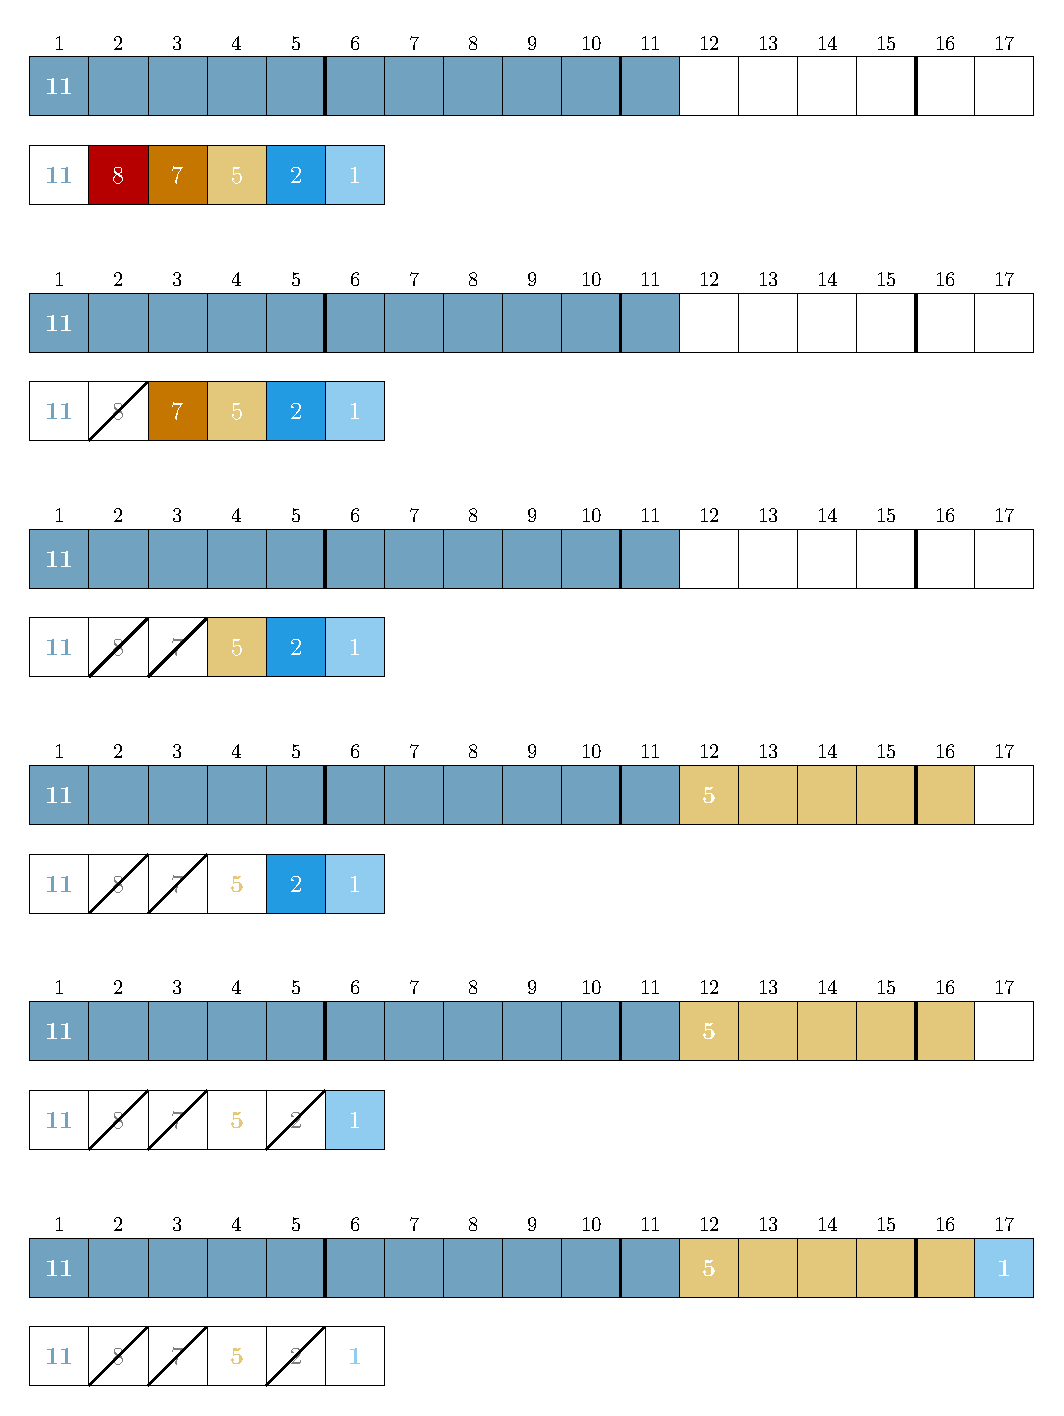
\includegraphics[width=0.6\linewidth]{ex1-6-GS.pdf}
    \caption{Solution de l'instance facile de l'exercice \ref{ex:ex1}}
  \end{figure}

    \begin{figure}[htbp]
    \centering
    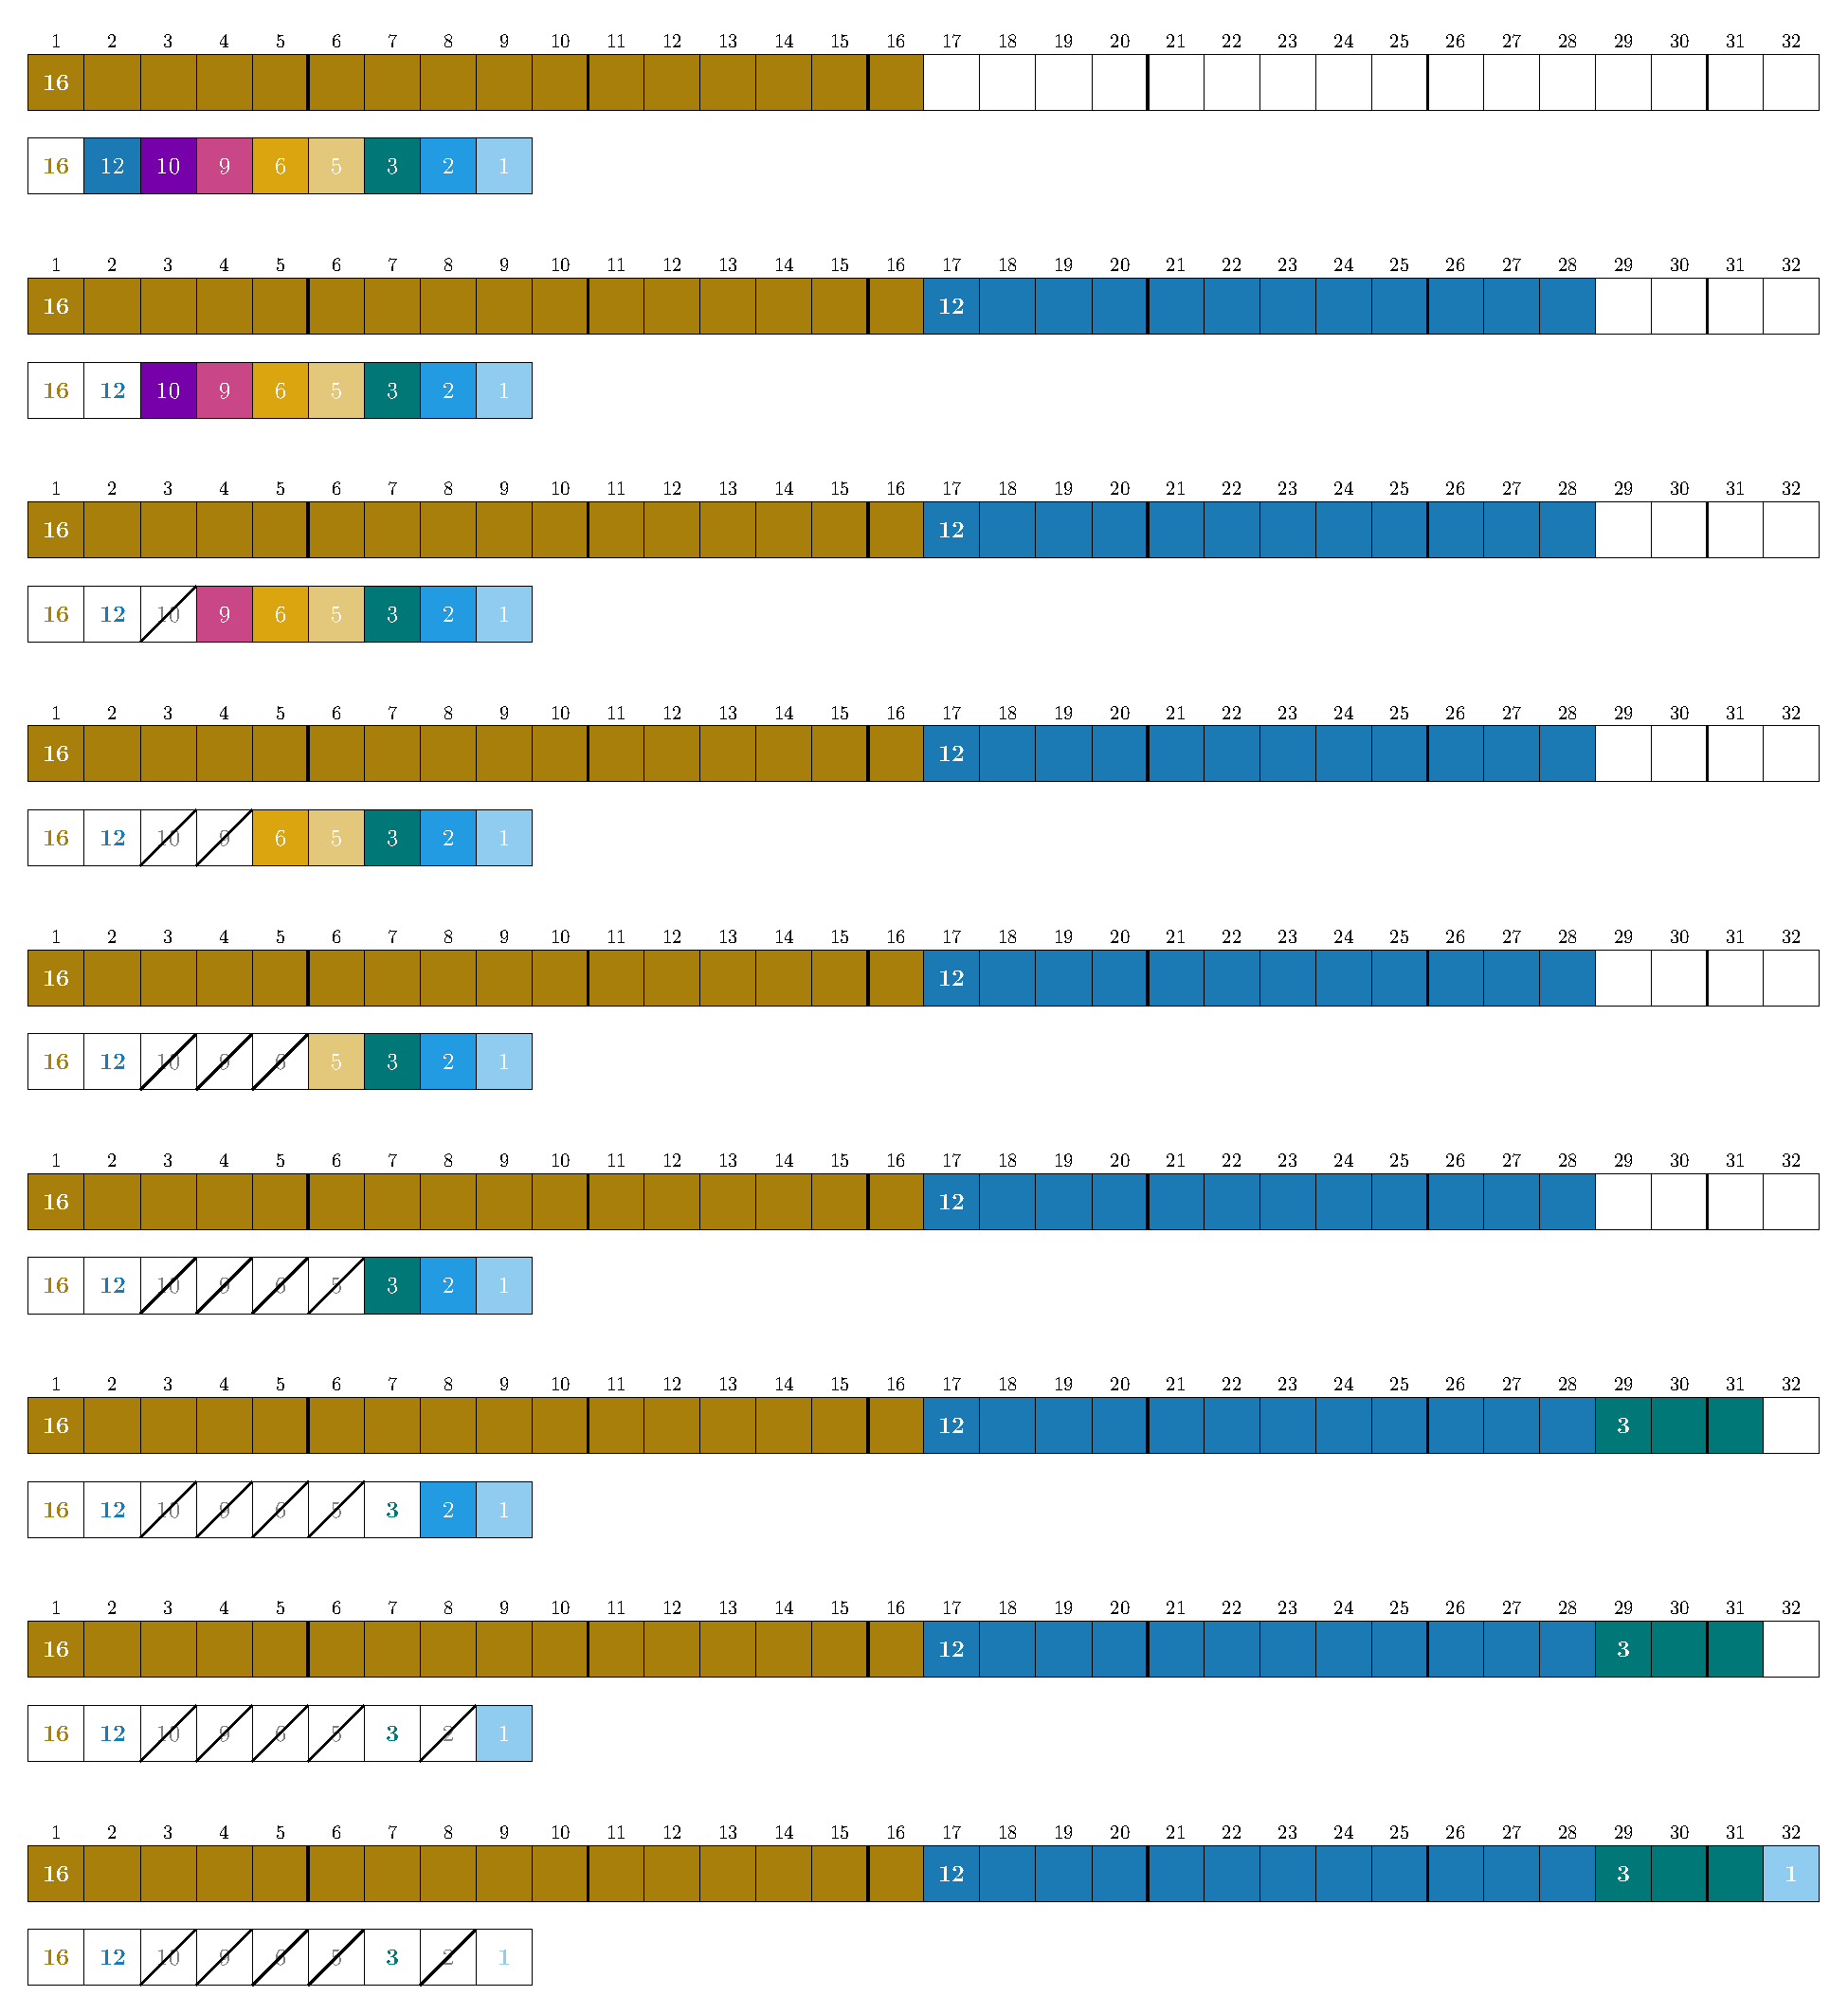
\includegraphics[width=0.6\linewidth]{ex1-9-GS.pdf}
    \caption{Solution de l'instance intermédiaire de l'exercice \ref{ex:ex1}}
  \end{figure}


  \begin{exercice}{}
    \label{ex:ex2}
    Appliquer l'algorithme glouton sur une instance.\\
    \begin{tabular}{lll}
      \toprule
      Niveau & Sac & Capacité \\
      \midrule
      Facile & 14, 13, 11, 7, 5, 3 & 26 \\
      Intermédiaire & 16, 15, 14, 13, 12, 9, 8, 6, 1 & 47 \\
      Difficile & ? & ? \\
      \bottomrule
      \end{tabular}
  \end{exercice}

  \begin{figure}[htbp]
    \centering
    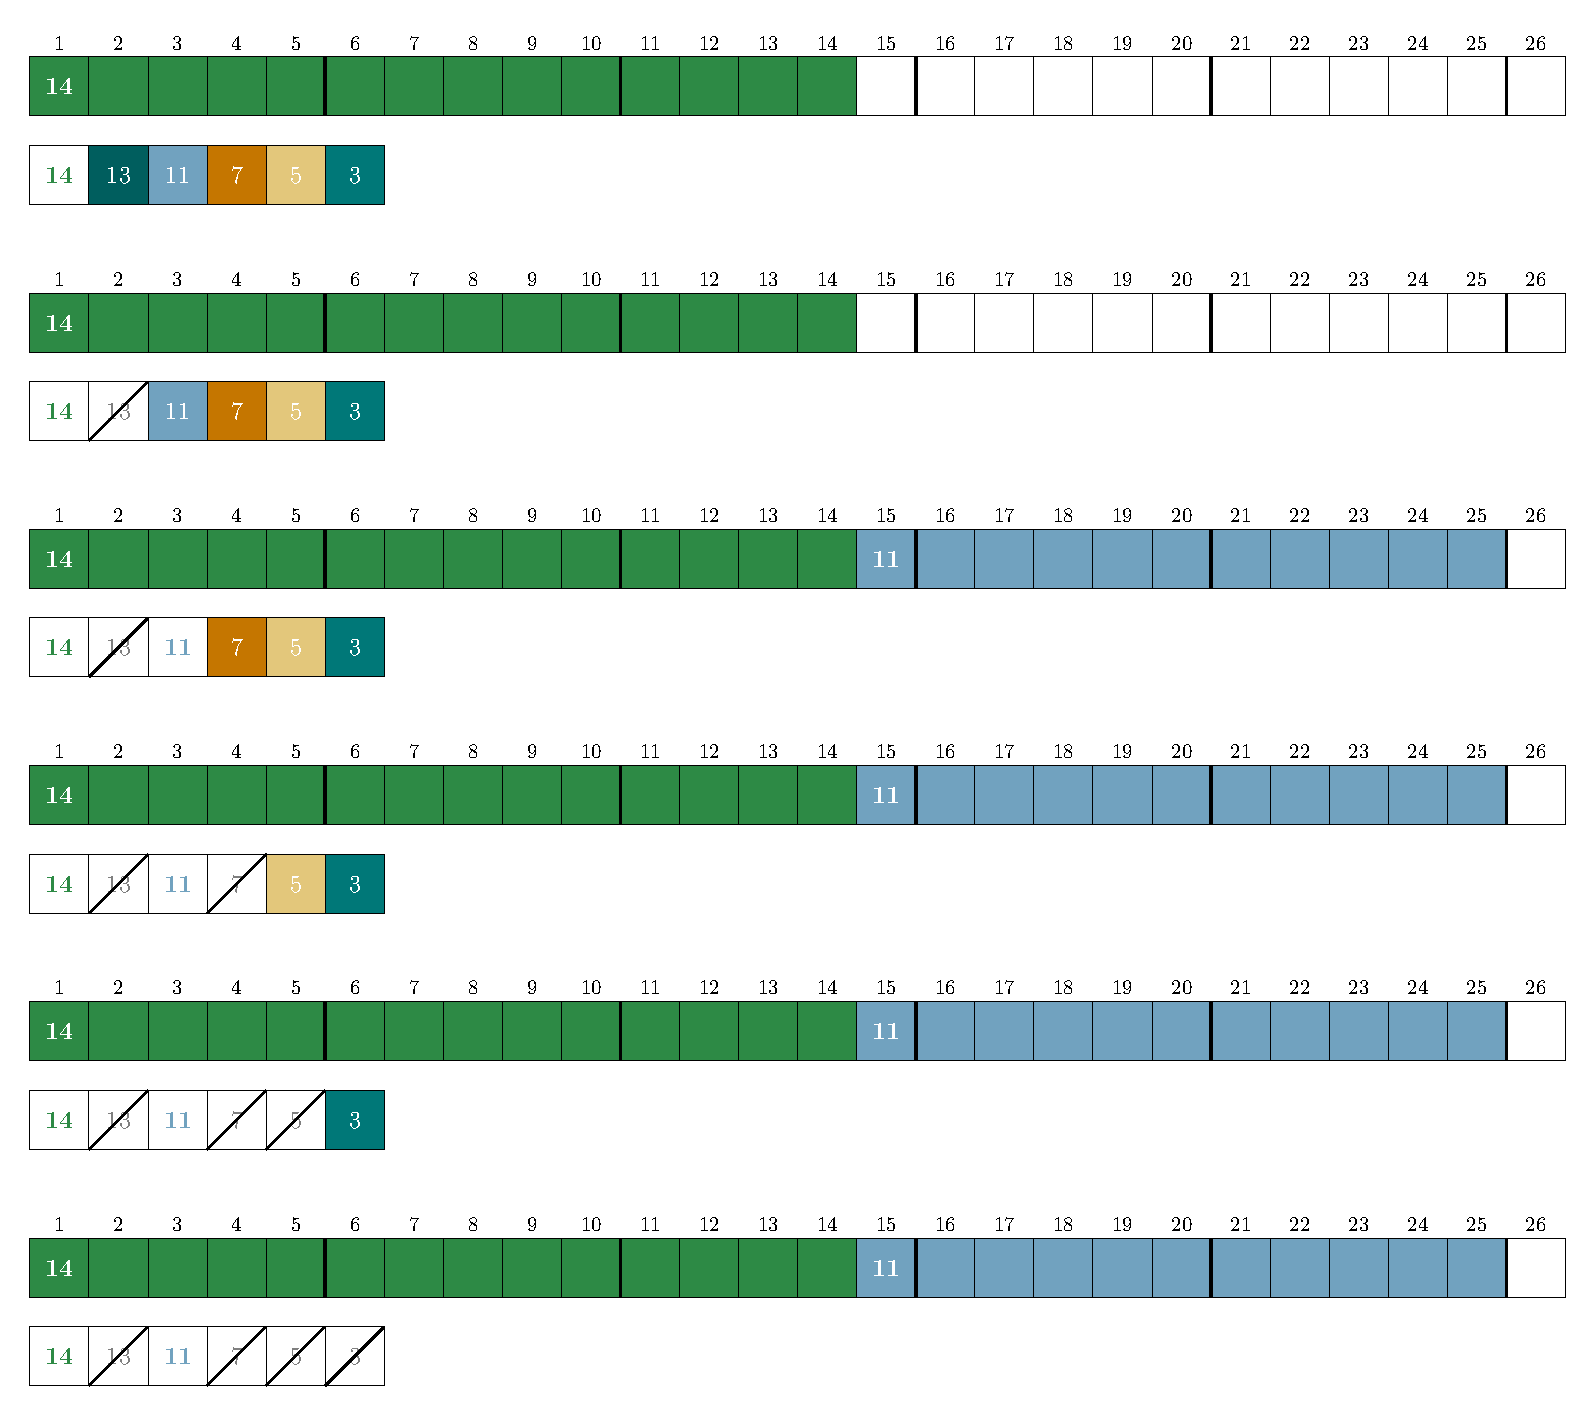
\includegraphics[width=0.6\linewidth]{ex2-6-GS.pdf}
    \caption{Solution de l'instance facile de l'exercice~\ref{ex:ex2}}
  \end{figure}

  \begin{figure}[htbp]
    \centering
    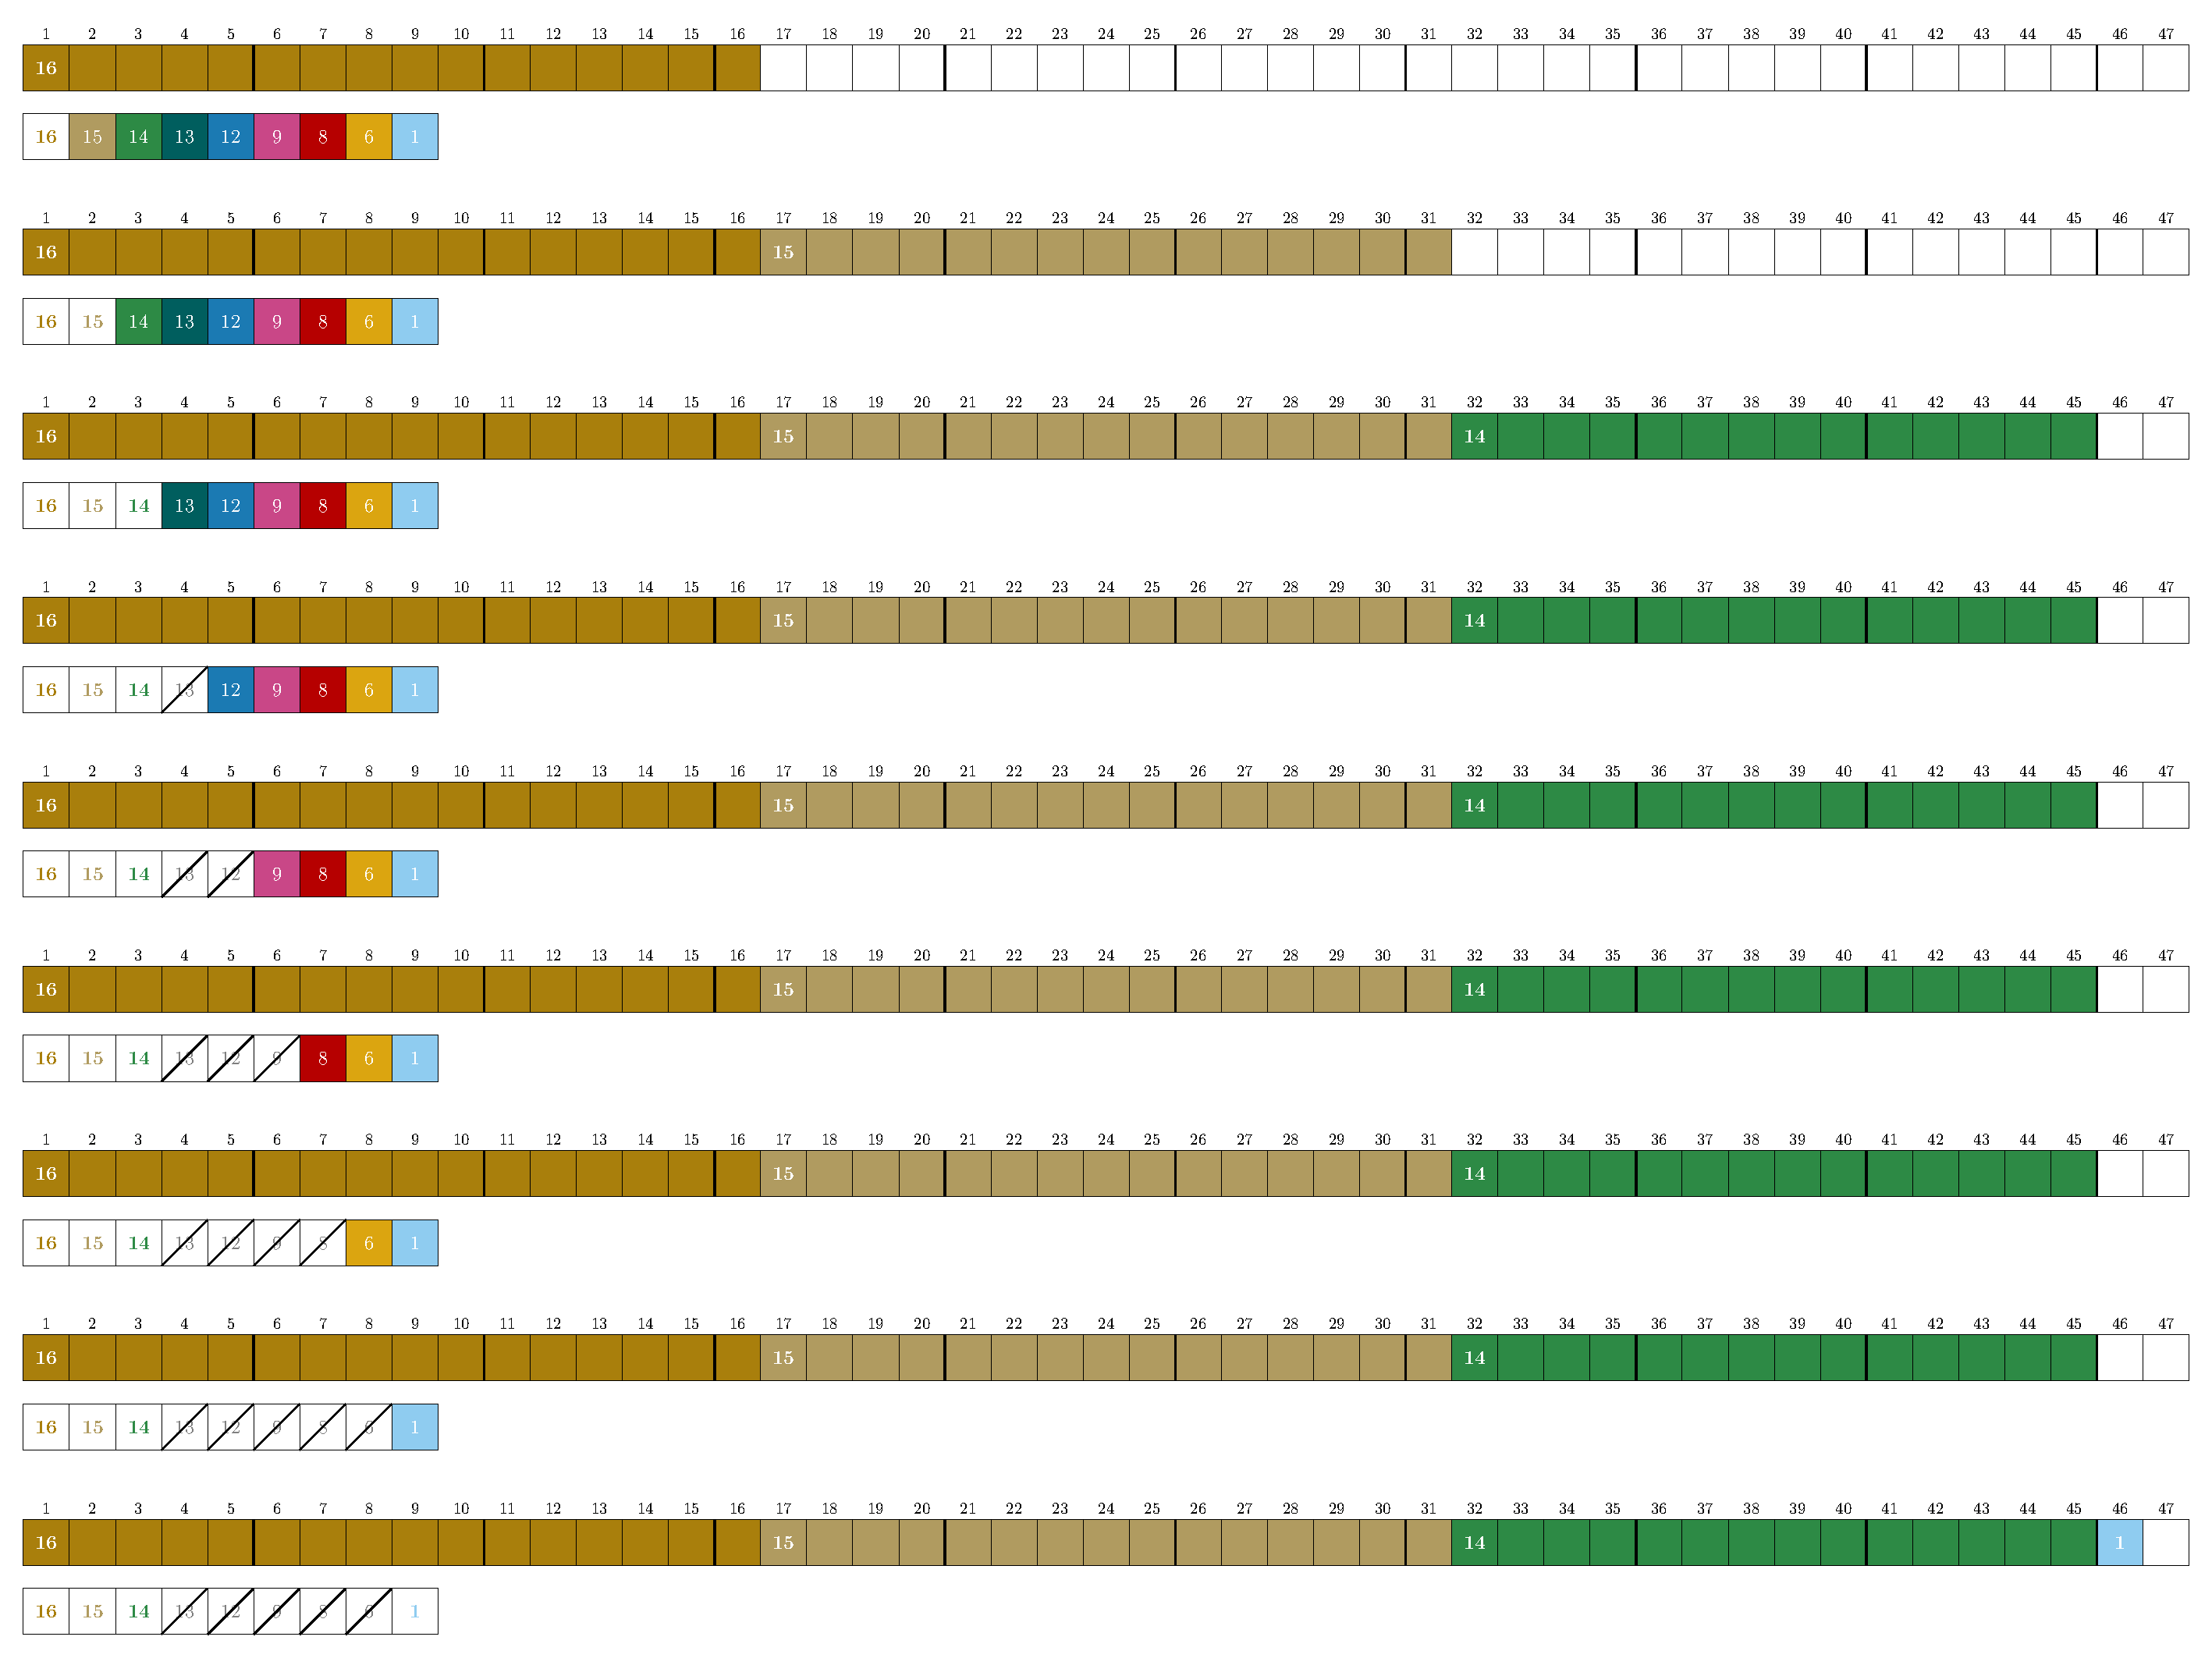
\includegraphics[width=0.6\linewidth]{ex2-9-GS.pdf}
    \caption{Solution de l'instance intermédiaire de l'exercice~\ref{ex:ex2}}
  \end{figure}


  \begin{algorithme}{Algorithme glouton répété}
     \label{ex:ex3}
    Répéter jusqu'à ce que le sac soit rempli ou contienne tous les objets :
    \begin{itemize}
    \item Appliquer l'algorithme glouton.
    \item Éliminer le plus grand objet
    \end{itemize}
  \end{algorithme}

  \begin{exercice}{}
    Appliquer l'algorithme glouton sur une instance de l'exercice~\ref{ex:ex2}.
  \end{exercice}
 \begin{figure}[htbp]
    \centering
    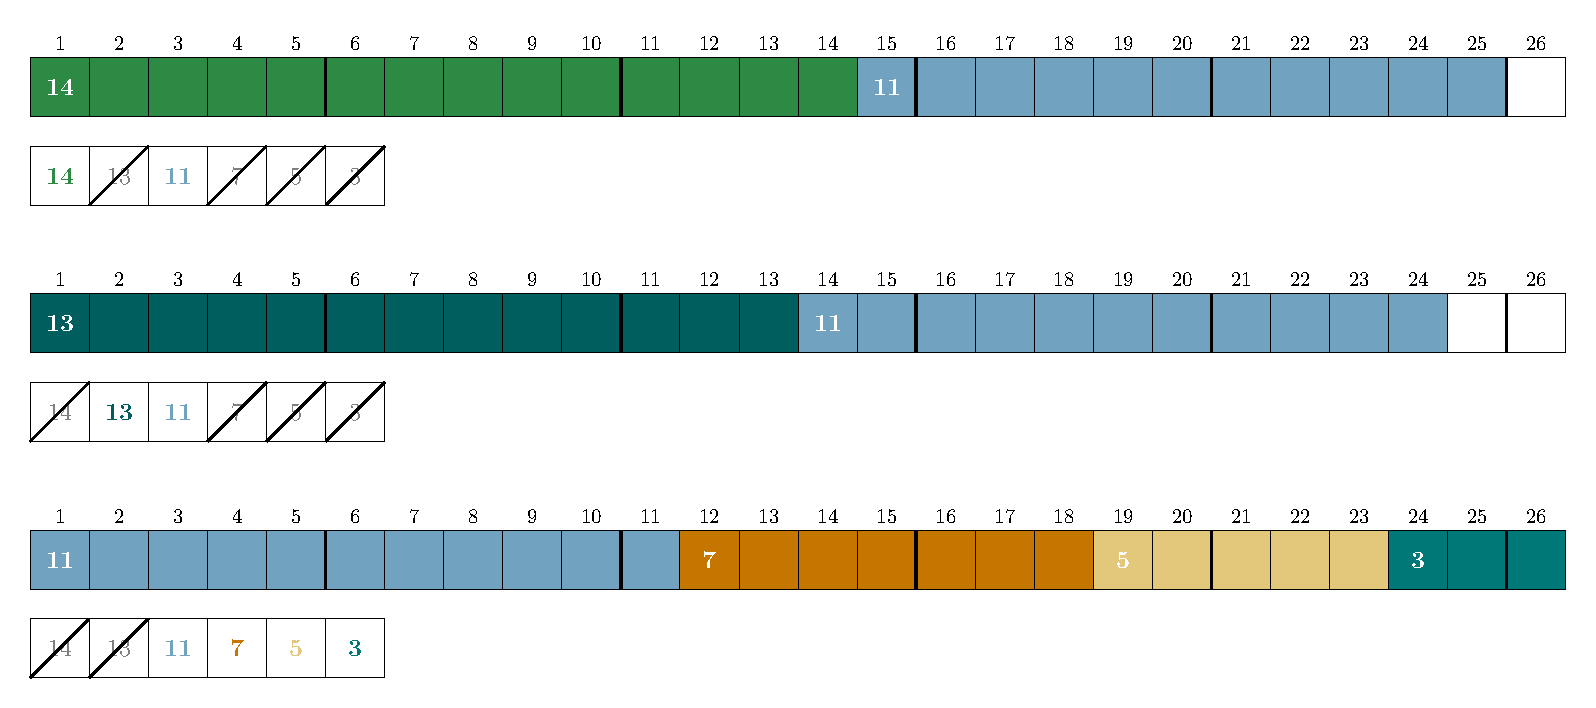
\includegraphics[width=0.6\linewidth]{ex2-6-MTGS.pdf}
    \caption{Solution de l'instance facile de l'exercice~\ref{ex:ex3}}
  \end{figure}

  \begin{figure}[htbp]
    \centering
    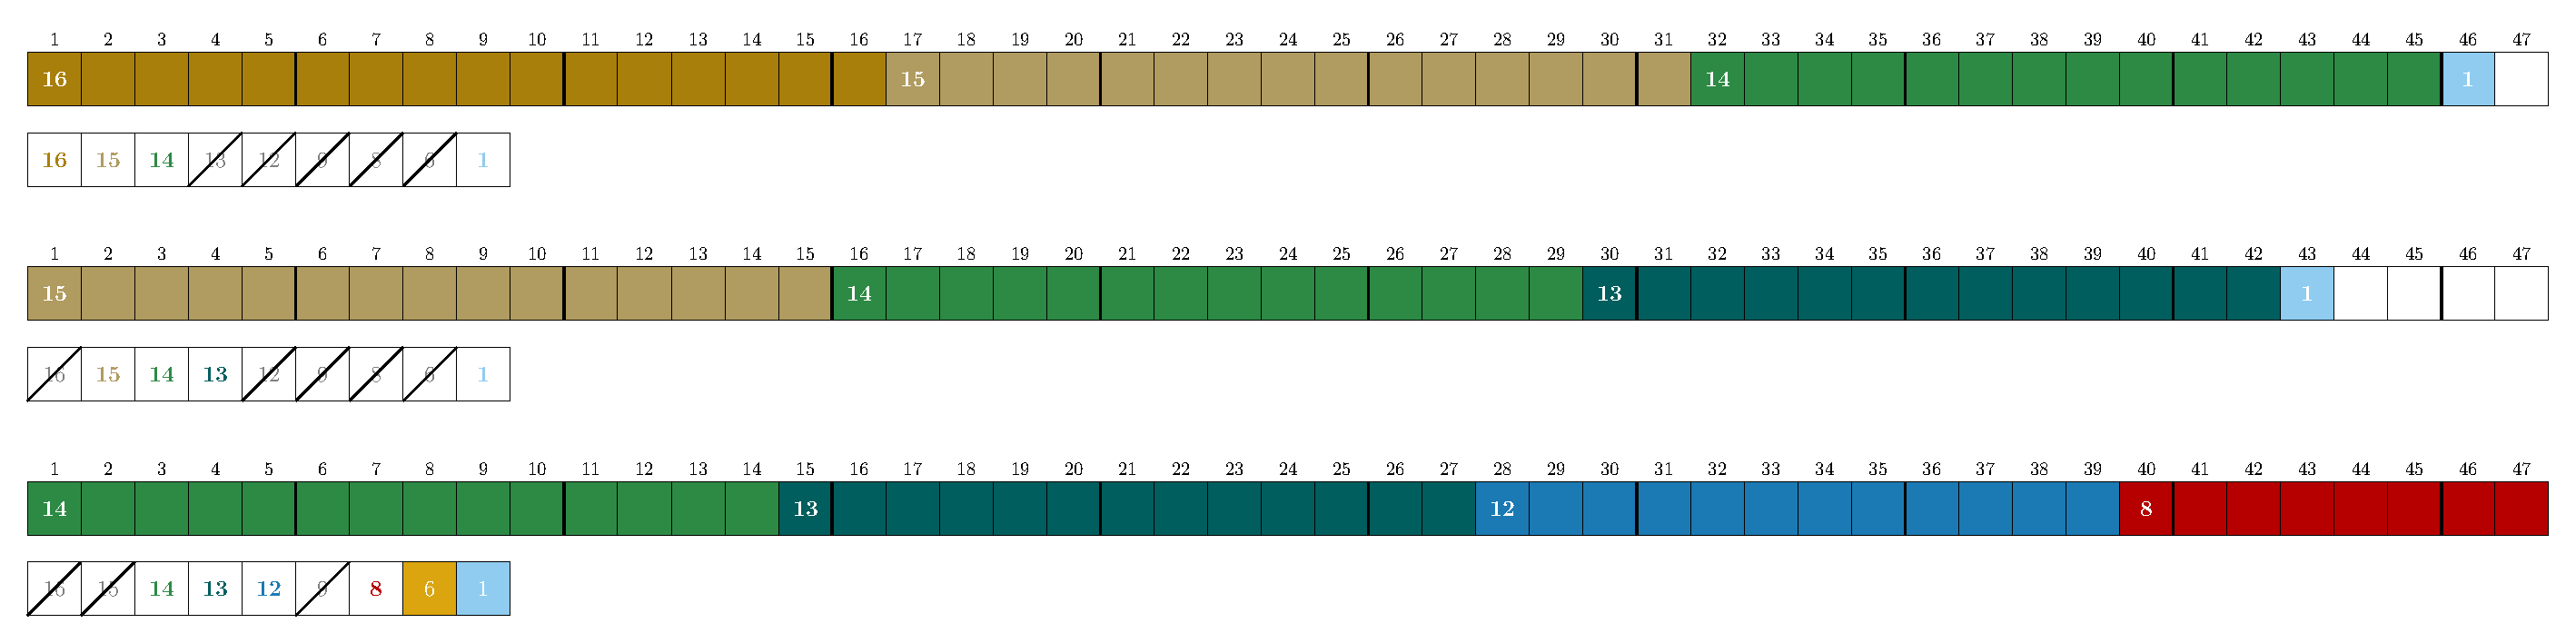
\includegraphics[width=0.6\linewidth]{ex2-9-MTGS.pdf}
    \caption{Solution de l'instance intermédiaire de l'exercice \ref{ex:ex3}}
  \end{figure}


   \begin{exercice}{}
    \label{ex:ex4}
    Appliquer l'algorithme glouton répété sur une instance.\\
    \begin{tabular}{lll}
      \toprule
      Niveau & Sac & Capacité \\
      \midrule
      Facile & 13, 11, 9, 8, 6, 4 & 25 \\
      Intermédiaire & 16, 15, 14, 10, 9, 8, 6, 5, 3 & 43 \\
      Difficile & ? & ? \\
      \bottomrule
      \end{tabular}
  \end{exercice}

 \begin{figure}[htbp]
    \centering
    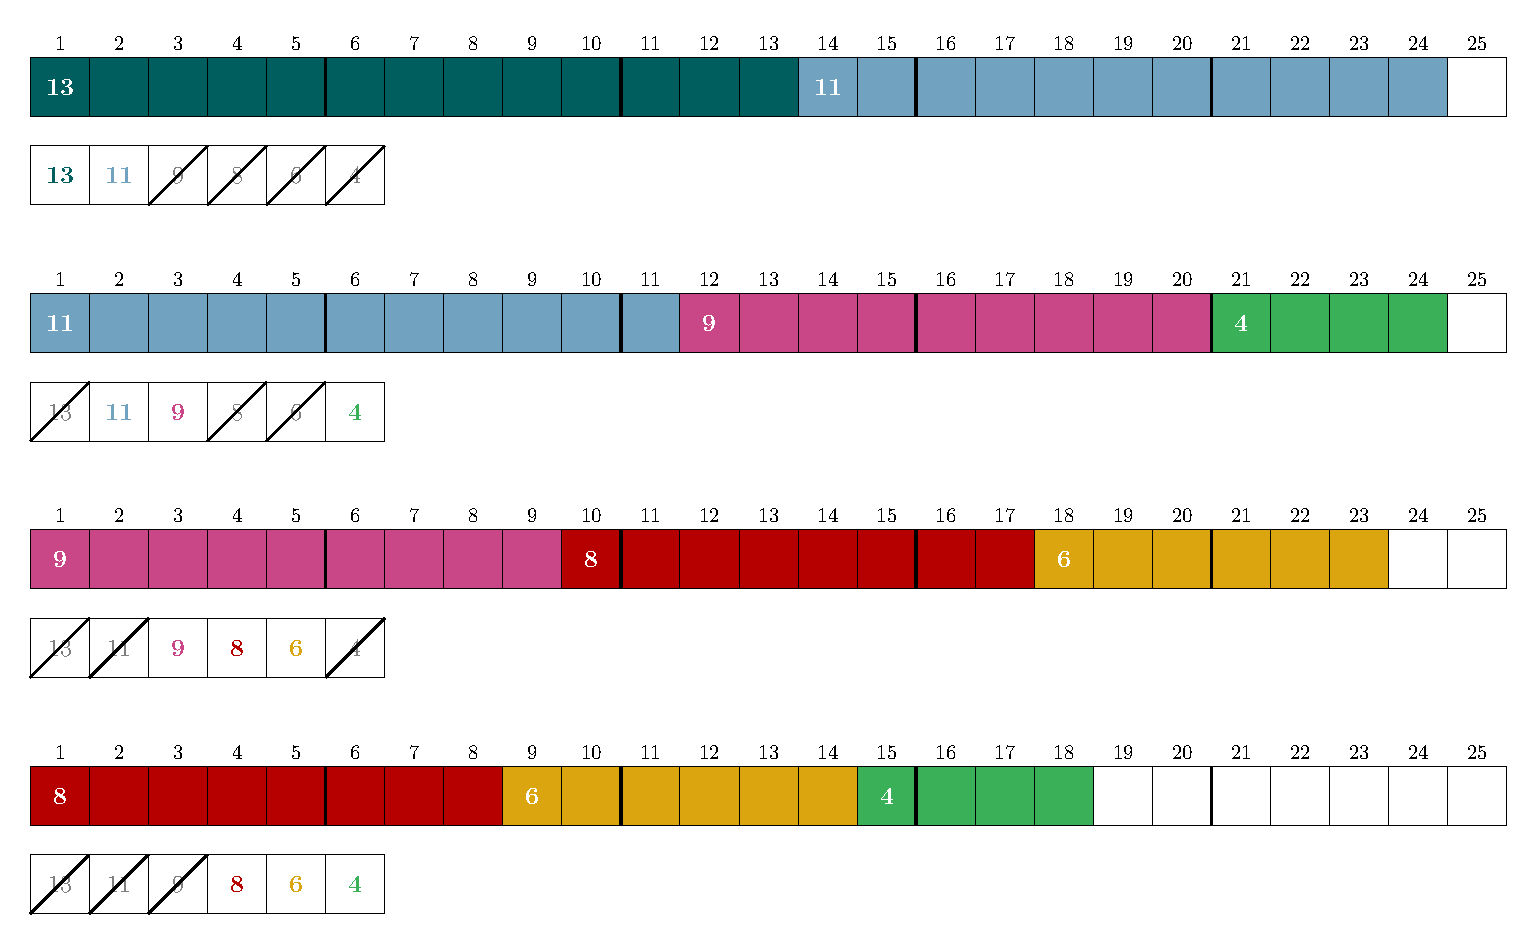
\includegraphics[width=0.6\linewidth]{ex3-6-MTGS.pdf}
    \caption{Solution de l'instance facile de l'exercice~\ref{ex:ex4}}
  \end{figure}

  \begin{figure}[htbp]
    \centering
    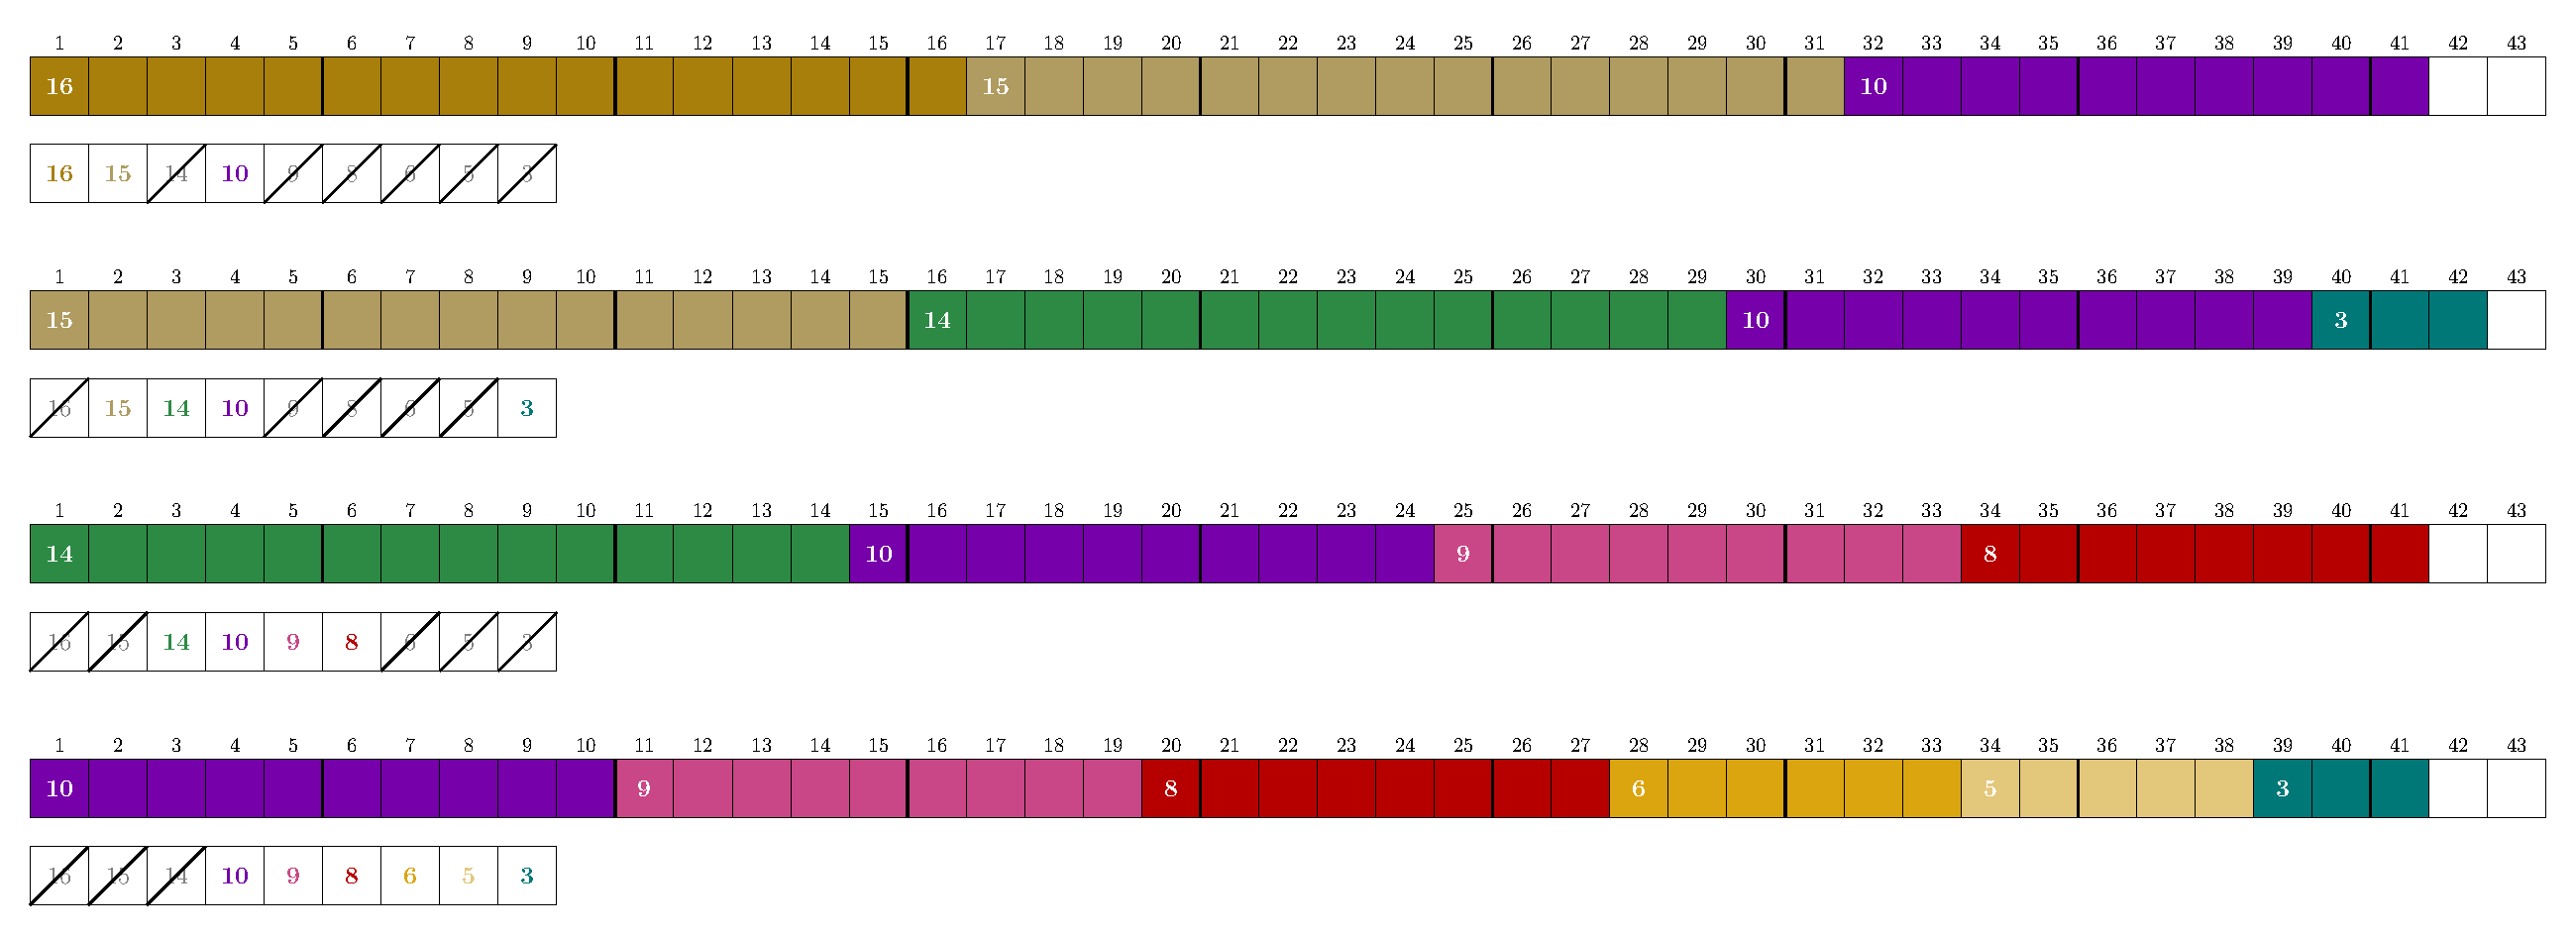
\includegraphics[width=0.6\linewidth]{ex3-9-MTGS.pdf}
    \caption{Solution de l'instance intermédiaire de l'exercice \ref{ex:ex4}}
  \end{figure}


  \section{Méthodes exactes}


  \begin{algorithme}{Algorithme de programmation dynamique}

    \end{itemize}
  \end{algorithme}


   \begin{exercice}{}
    \label{ex:ex3}
    Appliquer la programmation dynamique sur une instance de l'exercice~\ref{ex:ex4}.\\
  \end{exercice}

\begin{figure}[htbp]
    \centering
    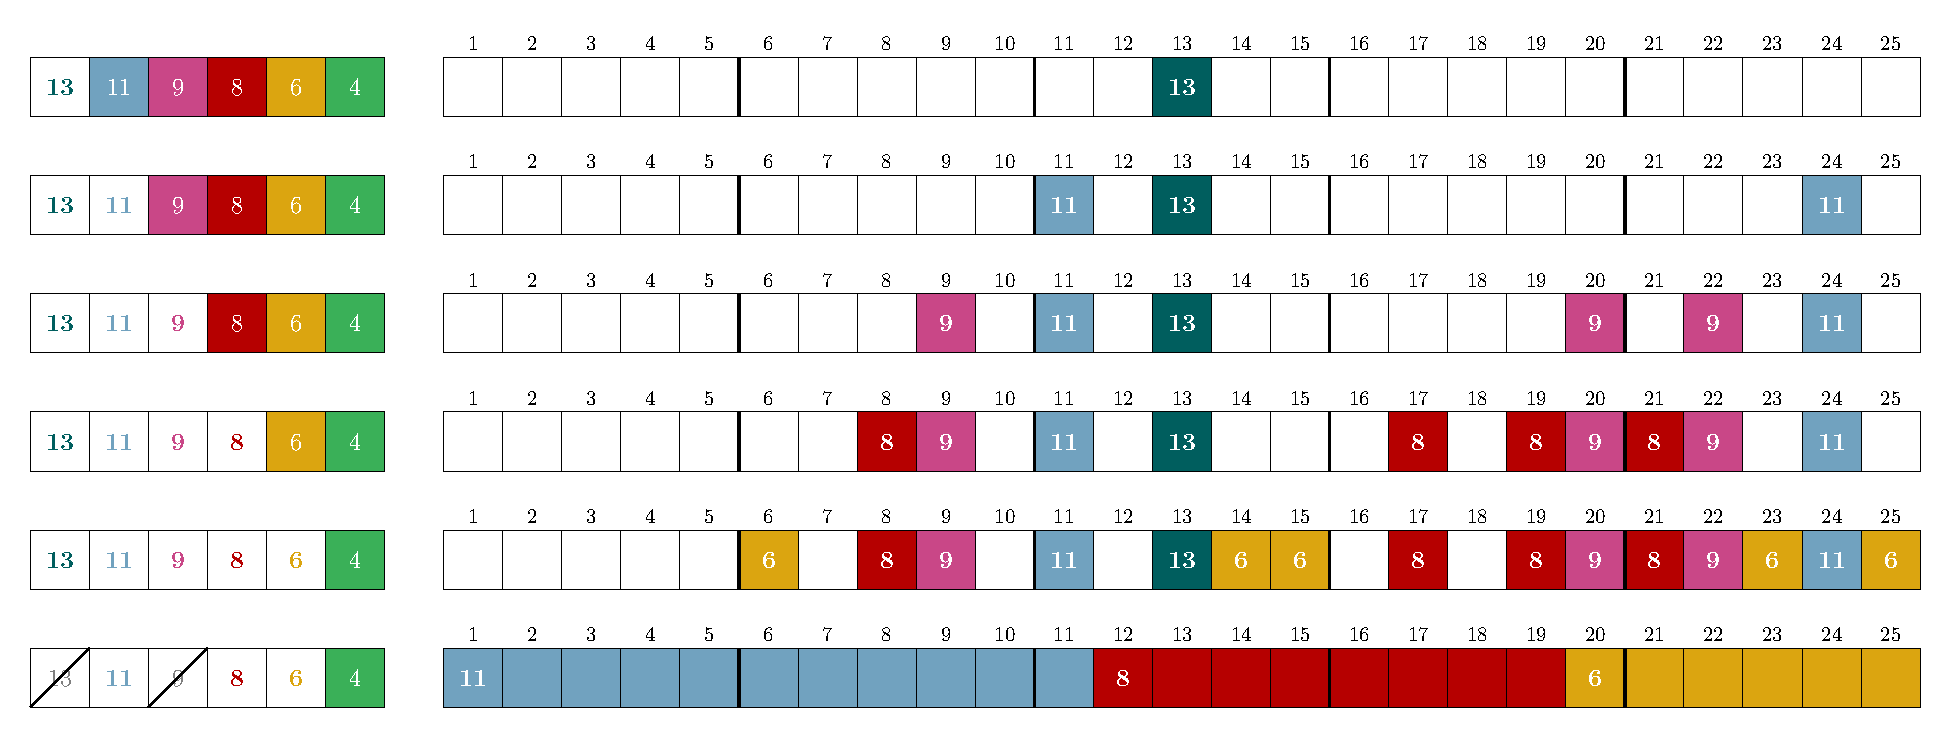
\includegraphics[width=0.6\linewidth]{ex3-6-DP.pdf}
    \caption{Solution de l'instance facile de l'exercice~\ref{ex:ex4}}
  \end{figure}

  \begin{figure}[htbp]
    \centering
    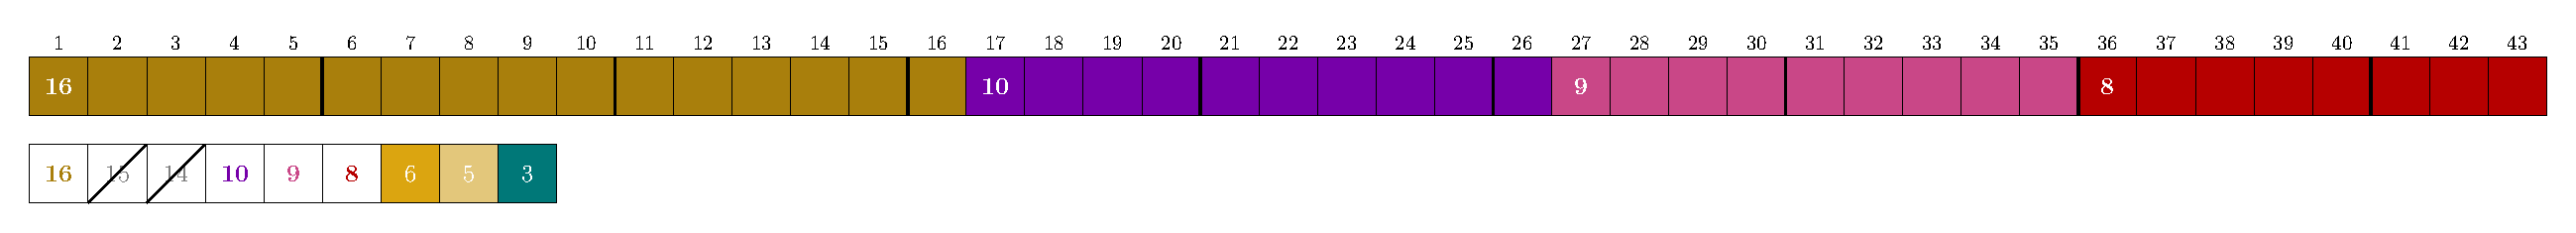
\includegraphics[width=0.6\linewidth]{ex3-9-DP.pdf}
    \caption{Solution de l'instance intermédiaire de l'exercice \ref{ex:ex4}}
  \end{figure}

\begin{figure}[htbp]
    \centering
    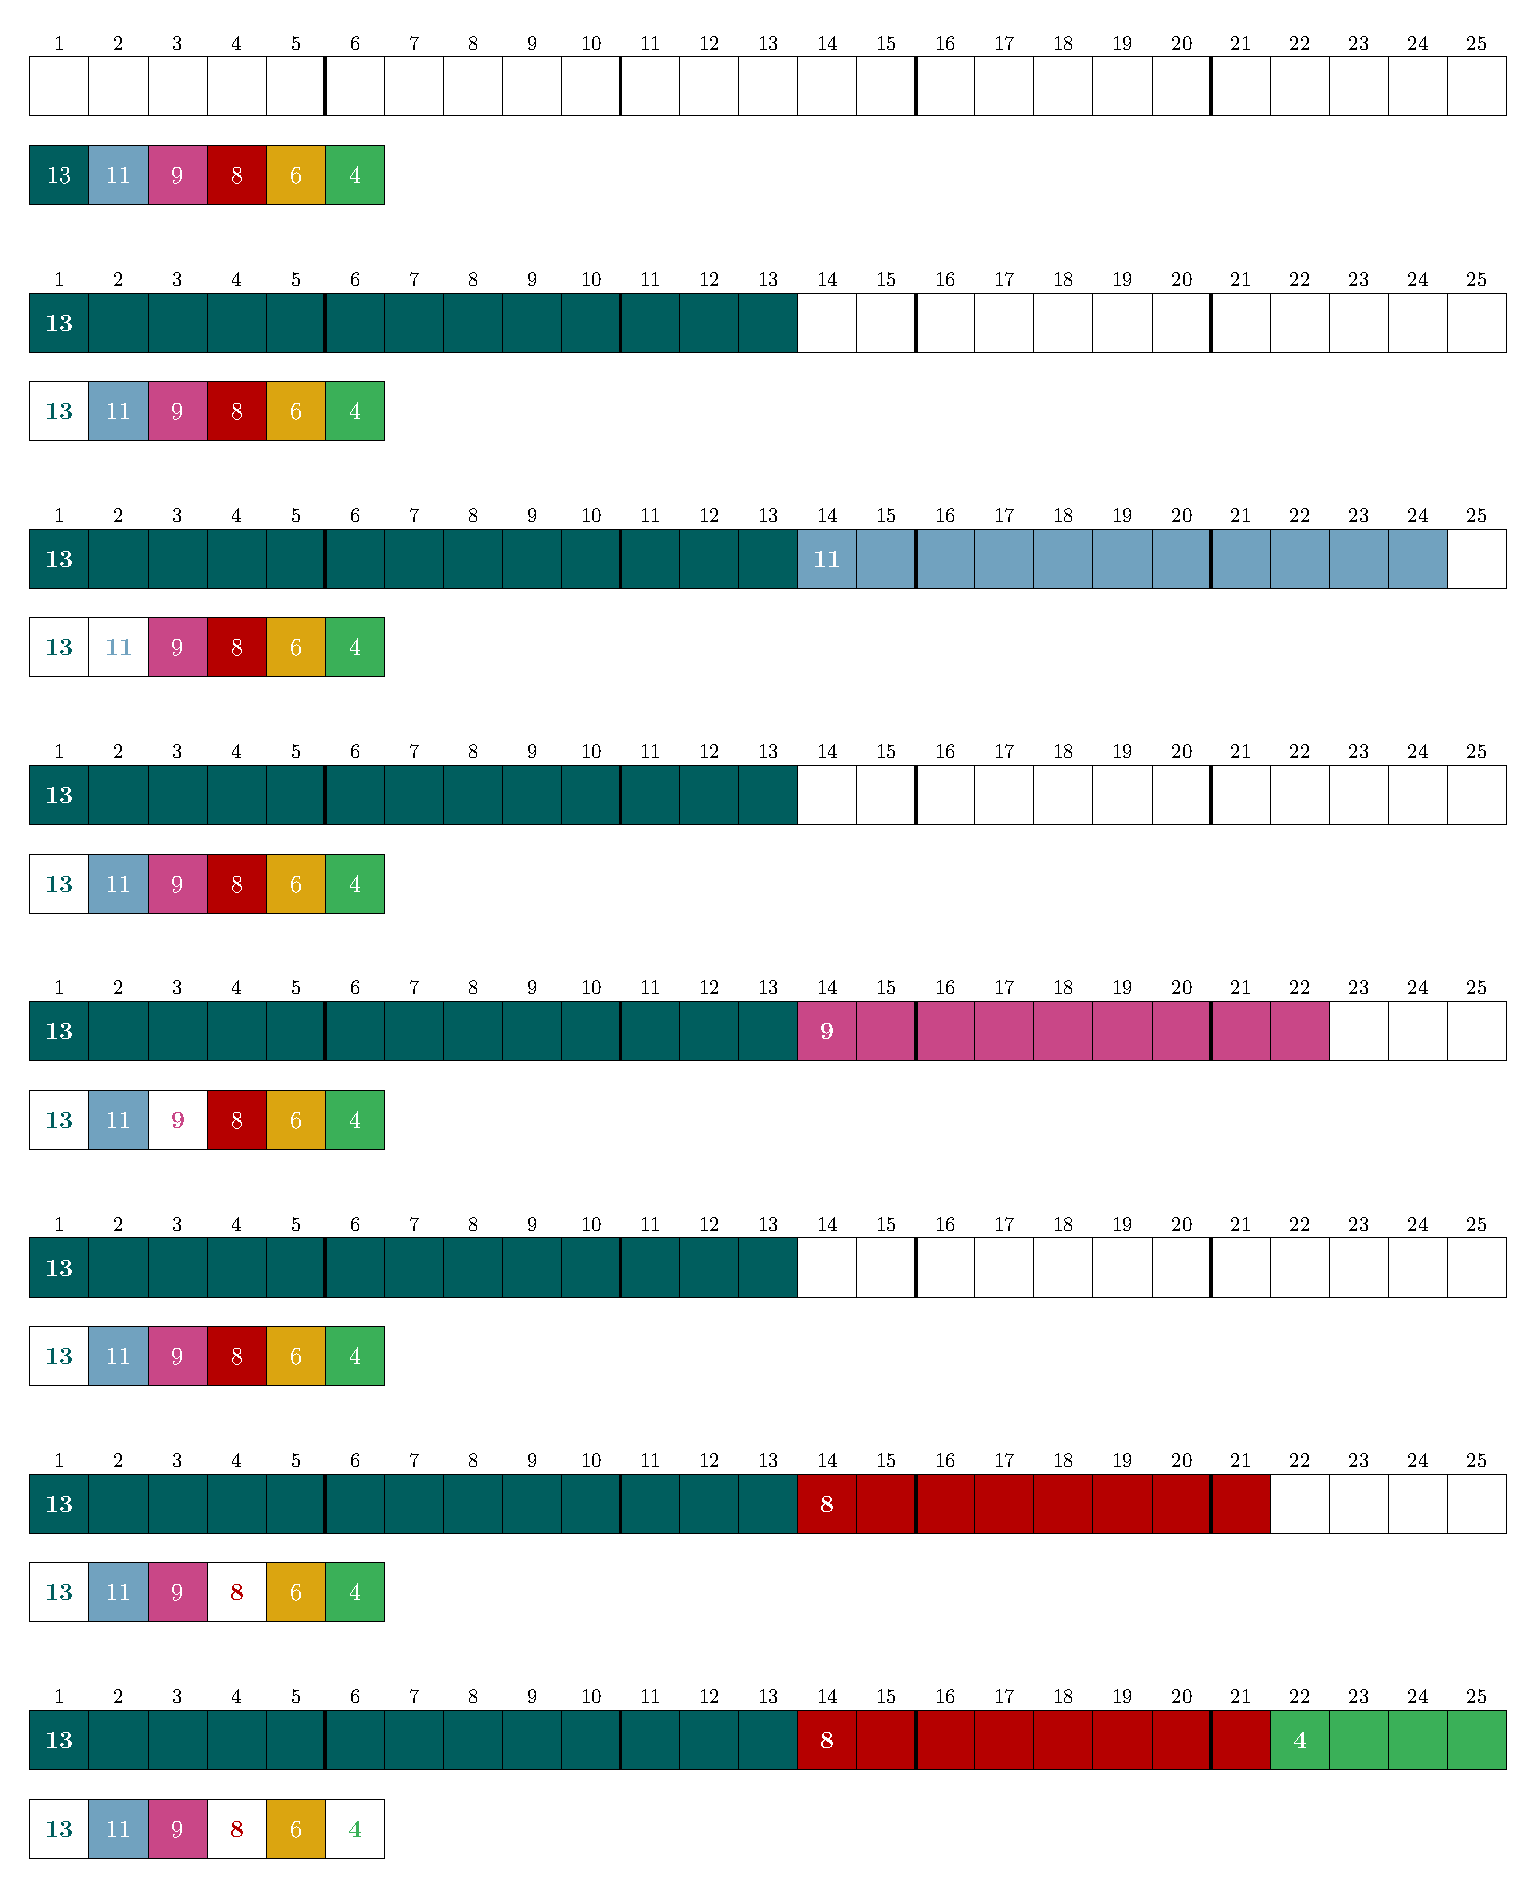
\includegraphics[width=0.6\linewidth]{ex3-6-TG.pdf}
    \caption{Solution de l'instance facile de l'exercice~\ref{ex:ex4}}
  \end{figure}

  \begin{figure}[htbp]
    \centering
    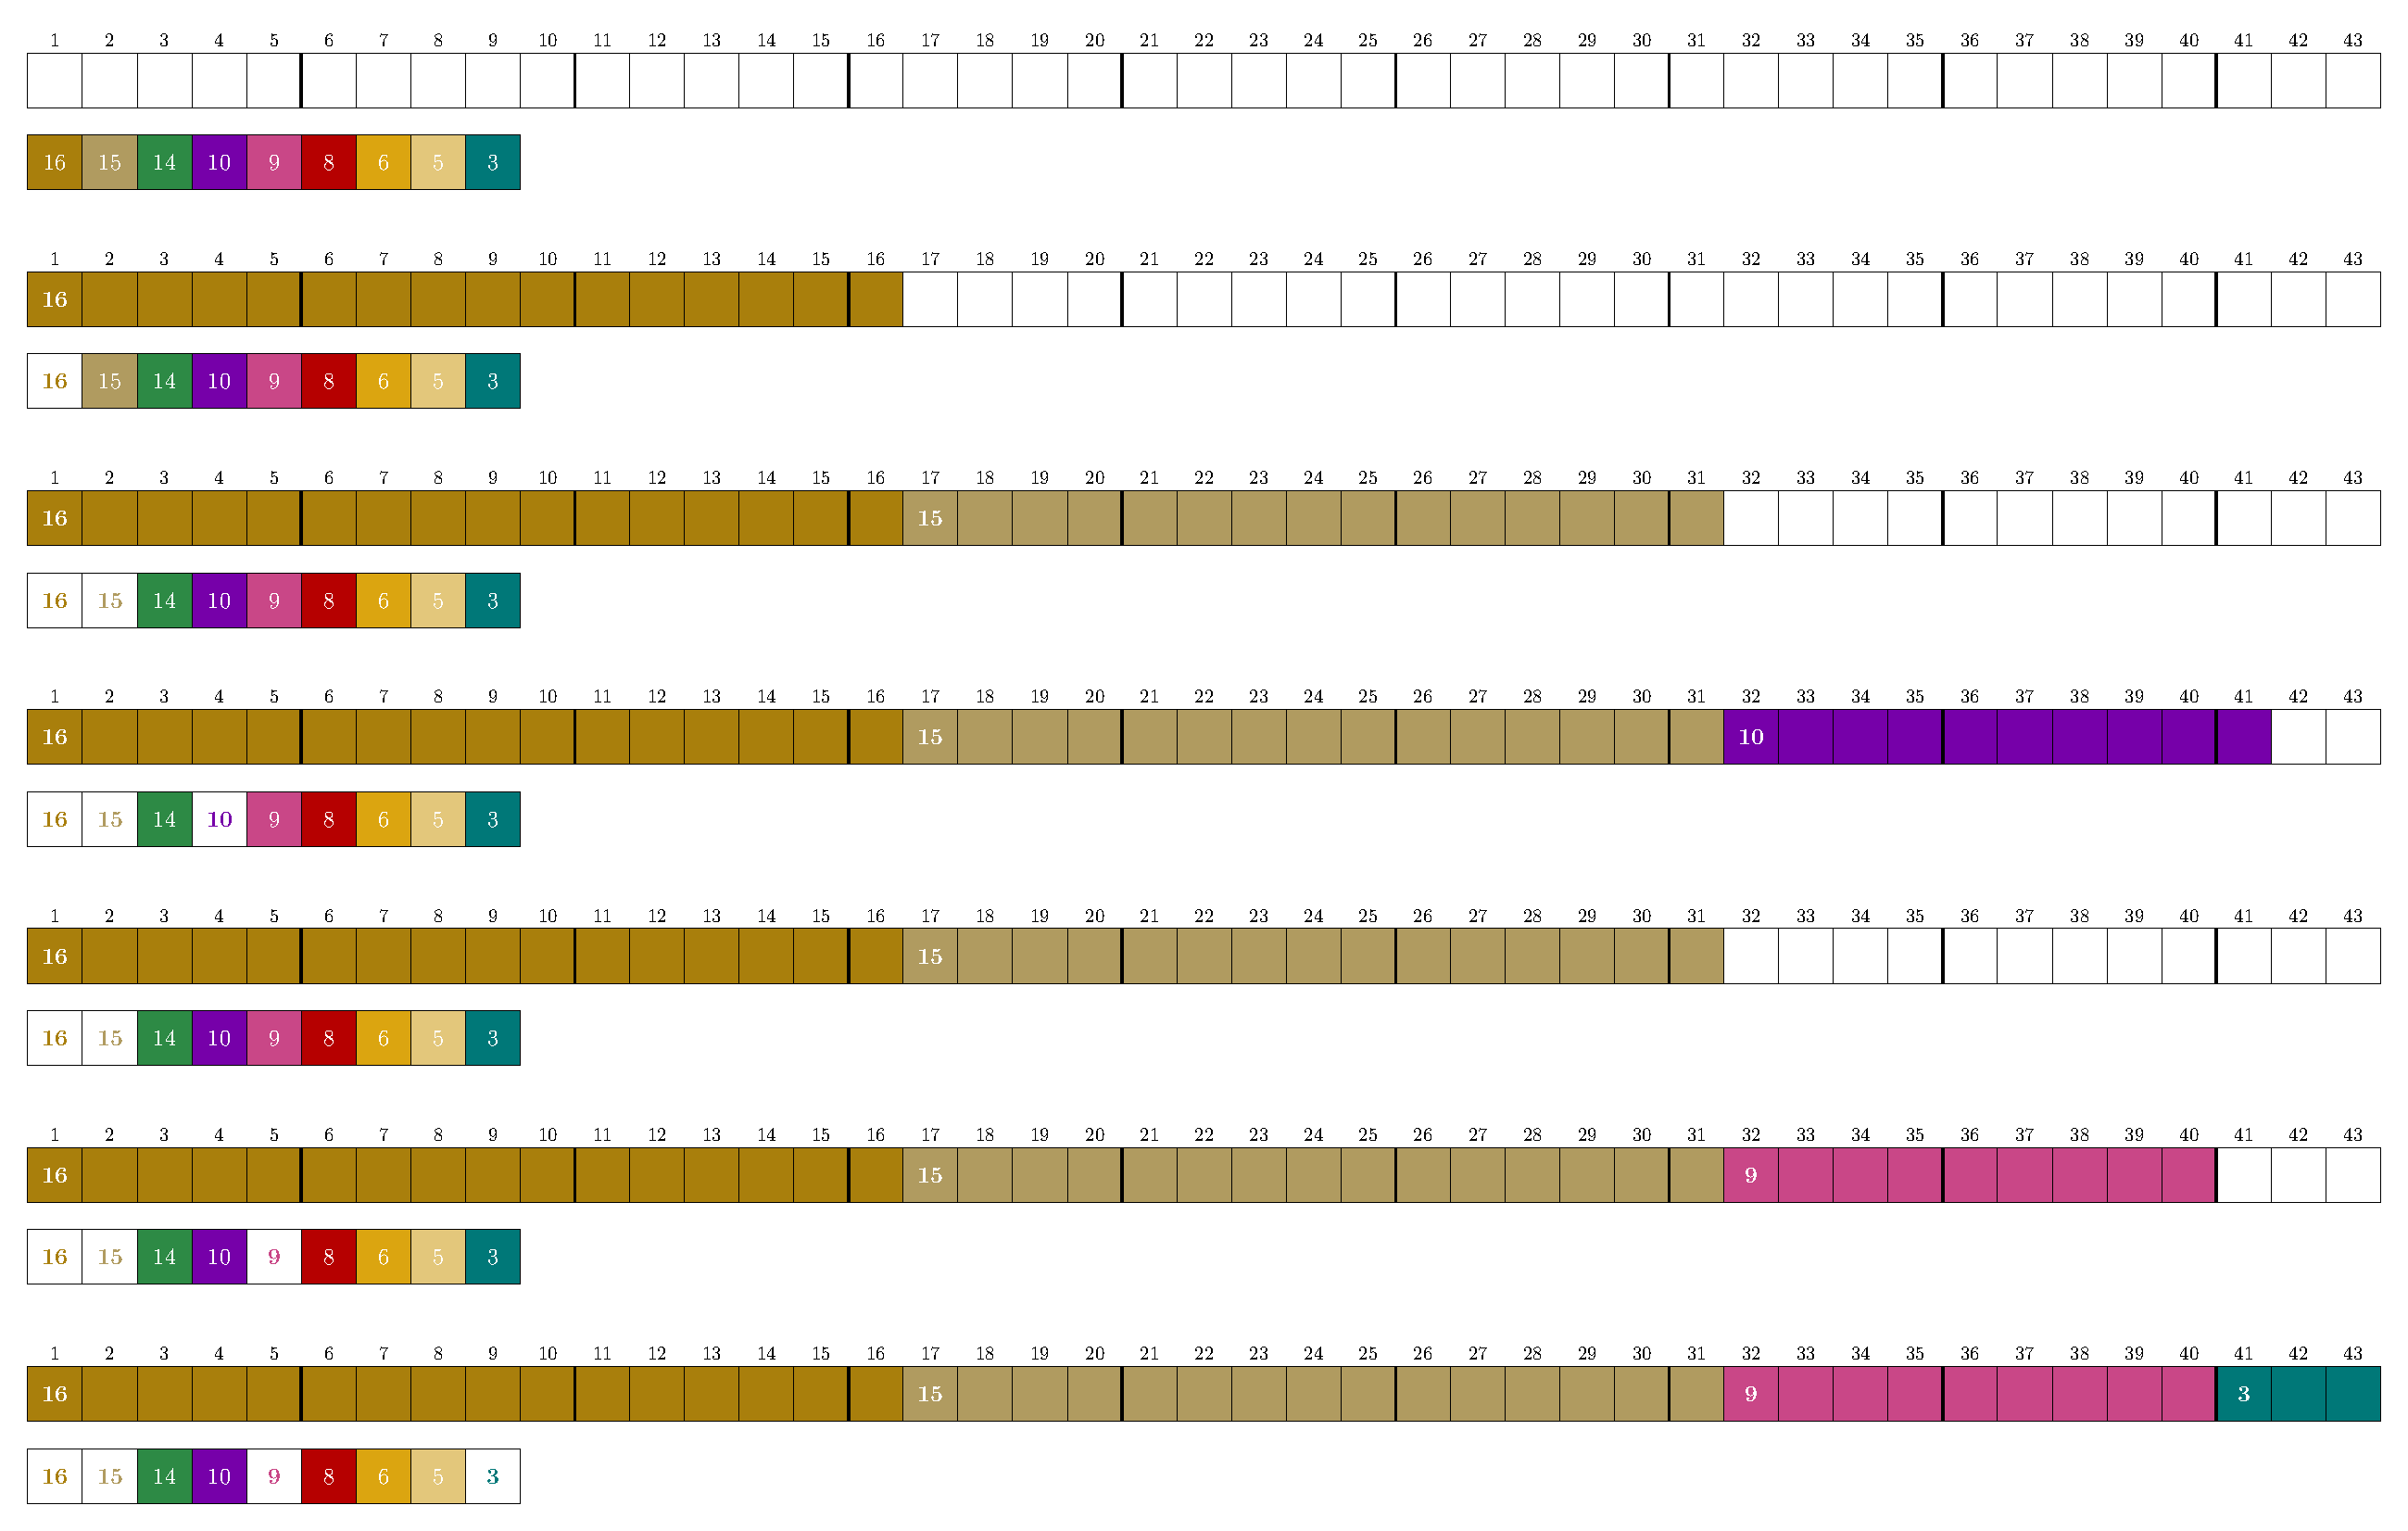
\includegraphics[width=0.6\linewidth]{ex3-9-TG.pdf}
    \caption{Solution de l'instance intermédiaire de l'exercice \ref{ex:ex4}}
  \end{figure}




    \begin{exercice}{}
    \label{ex:ex4}
    Appliquer la programmation dynamique sur une instance.\\
    \begin{tabular}{lll}
      \toprule
      Niveau & Sac & Capacité \\
      \midrule
      Facile & 16, 15, 11, 4, 2, 1 & 24 \\
      Intermédiaire & 18, 15, 13, 10, 8, 5, 3, 2 & 37 \\
      Difficile & ? & ? \\
      \bottomrule
      \end{tabular}
    \end{exercice}


    \begin{figure}[htbp]
    \centering
    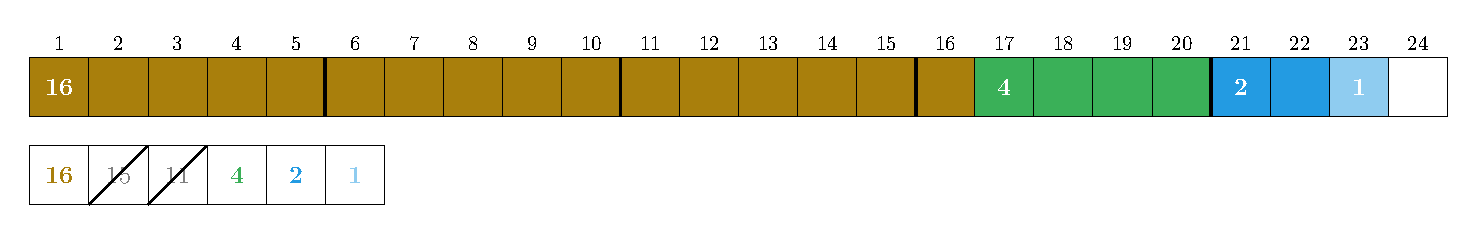
\includegraphics[width=0.6\linewidth]{ex4-6-DP.pdf}
    \caption{Solution de l'instance facile de l'exercice~\ref{ex:ex4}}
  \end{figure}

  \begin{figure}[htbp]
    \centering
    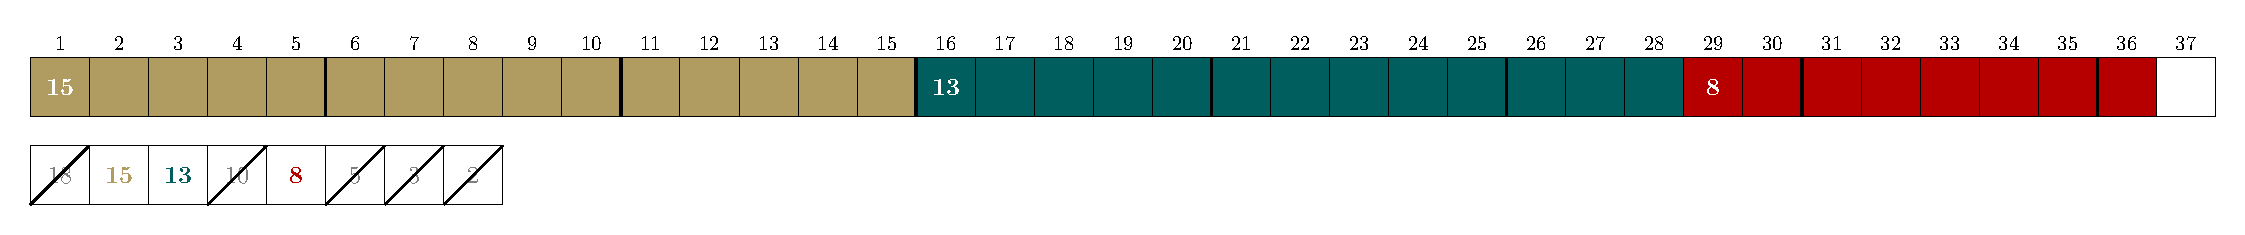
\includegraphics[width=0.6\linewidth]{ex4-8-DP.pdf}
    \caption{Solution de l'instance intermédiaire de l'exercice \ref{ex:ex4}}
  \end{figure}


  \subsection{Programmation dynamique}

  \subsection{Tester et Générer}

  \appendix
  \section{Problèmes connexes}

  % \subsection{Subset Sum Problem}
  % \cite{SSP}

  % \subsection{Ordonnancement}
  % \cite{MS}
  % \cite{Korf2013}

  % \subsection{Sac-à-dos}
  % \cite{KP}
  % \cite{MartelloToth1990}

  % \begin{tikzpicture}
  %   \filldraw [fill = bleuTN] (0, 2) rectangle (8, 3);
  %   \filldraw [fill = rouge] (8, 2) rectangle (14, 3);

  %   \draw [<->, very thick, exCol] (7, 3.25) -- (8, 3.25) node [right] {Ordonnancement};

  %   \filldraw [fill = rouge] (0, 0) rectangle (6, 1);
  %   \filldraw [fill = bleuTN] (6, 0) rectangle (14, 1);

  %   \draw [<->, very thick, orange] (7, -0.25) -- (6, -0.25) node [left] {Sac-à-dos};

  %   \draw [<->, very thick, violet] (6.5, 1.5) -- (7.5, 1.5) node [right] {Partition};

  %   \draw [dashed, very thick] (7, -0.75) -- (7, 3.75) node [above] {C};
  % \end{tikzpicture}




  \begin{algorithme}{}
    test
  \end{algorithme}


  \begin{plusloin}{}
    test
  \end{plusloin}

  \bibliographystyle{plain}
  \bibliography{poly}
\end{document}
